% Teil II: Mathematik lesen und sprechen.
% \lies{Ausdruck}{Japanisch in Kurzschreibweise}{deutsche Lesart}
% Die Kurzschreibweise (Wort|Lesung, durch Leerzeichen getrennt) steht in umschrift.py; bauen.py macht
% daraus \lies{Ausdruck}{Japanisch}{Umschrift}{deutsche Lesart}.
%%%%  TEIL B: MATHEMATIK LESEN UND SPRECHEN  %%%%
\newpage
\part{Mathematik lesen und sprechen}

In diesem Teil steht, wie man Zeichen, Formeln und Rechenwege auf Japanisch (und zum Vergleich auf
Deutsch) vorliest. Links steht der Ausdruck, rechts die japanische Lesart, darunter klein ihre
Umschrift und grau die deutsche Lesart. Wo es mehrere übliche Lesarten gibt, sind sie durch
Schrägstriche getrennt. Die Beispiele sind bewusst einfach gehalten, damit sie sich direkt im
Unterricht verwenden lassen.

\smallskip
Variablen wie $x$ bleiben in der Umschrift stehen; gesprochen werden sie mit ihren englischen
Buchstabennamen (\textit{ekkusu}, \textit{wai}). Terme und Gleichungen liest man im Unterricht meist
mit den Lehnwörtern \jp{プラス}{purasu}, \jp{マイナス}{mainasu} und \jp{イコール}{ikōru}. Beim Rechnen
mit Zahlen sind auch die japanischen Wörter \jp{足す}{tasu}, \jp{引く}{hiku}, \jp{掛ける}{kakeru} und
\jp{割る}{waru} üblich; „gleich“ heißt dann einfach \jp{は}{wa}.

%--------------------------------------------------------------------------------------------------
\section{Zahlen, Zeichen und Schreibweisen}

\subsection*{Ordnungszahlen, Indizes und Aufzählungen}

\begin{lesen}
\lies{1.\quad 2.\quad 3.\quad 21.}{第|だい 1|いち 、 第|だい 2|に 、 第|だい 3|さん 、 第|だい 21|にじゅういち / 1番目|いちばんめ 、 2番目|にばんめ 、 3番目|さんばんめ}{erstens, zweitens, drittens -- der Erste, der Zweite, \ldots}
\lies{1.\ \ldots, 2.\ \ldots}{第一|だいいち に \ldots 、 第二|だいに に \ldots}{erstens \ldots, zweitens \ldots}
\lies{$x_1,\ x_2$}{$x$ 1|いち 、 $x$ 2|に}{$x$ eins, $x$ zwei \;/\; $x$ Index eins}
\lies{$a_n$}{$a$ $n$ （ 添え字|そえじ は $n$ ）}{$a$ Index $n$ \;/\; $a$ $n$}
\lies{$1;\ 2;\ 3;\ \ldots$}{1|いち 、 2|に 、 3|さん 、 \ldots\ と 限りなく|かぎりなく 続く|つづく}{eins, zwei, drei und so weiter (unbegrenzt)}
\lies{$1;\ 2;\ \ldots;\ 25$}{1|いち 、 2|に 、 \ldots 、 25|にじゅうご まで}{eins, zwei und so weiter bis fünfundzwanzig}
\end{lesen}

\subsection*{Dezimalzahlen, große Zahlen und Brüche}

Im Japanischen trennt wie im Englischen ein \textbf{Punkt} die Nachkommastellen ab, das Komma gliedert
große Zahlen in Dreiergruppen -- im Deutschen ist es genau umgekehrt. Brüche liest man von unten nach
oben: erst den Nenner, dann \jp{分の}{bun no} und den Zähler.

\begin{lesen}
\lies{$3{,}14$ \newline \footnotesize jap. 3.14}{3.14|さん_てん_いち_よん}{drei Komma eins vier}
\lies{$0{,}3$ \newline \footnotesize jap. 0.3}{0.3|れい_てん_さん}{null Komma drei}
\lies{$30\,000$ \newline \footnotesize jap. 30,000}{3万|さんまん}{dreißigtausend}
\lies{$2{,}5 \cdot 10^6$ \newline \footnotesize jap. $2.5 \times 10^6$}{2.5|に_てん_ご 掛ける|かける 10|じゅう の 6乗|ろくじょう}{zwei Komma fünf mal zehn hoch sechs}
\lies{$\frac12;\ \frac13;\ \frac14$}{2|に 分|ぶん の 1|いち 、 3|さん 分|ぶん の 1|いち 、 4|よん 分|ぶん の 1|いち}{ein Halb, ein Drittel, ein Viertel}
\lies{$\frac34;\ \frac58$}{4|よん 分|ぶん の 3|さん 、 8|はち 分|ぶん の 5|ご}{drei Viertel, fünf Achtel}
\lies{$\frac{1}{100}$}{100|ひゃく 分|ぶん の 1|いち}{ein Hundertstel}
\lies{$\frac{17}{25}$}{25|にじゅうご 分|ぶん の 17|じゅうなな}{siebzehn Fünfundzwanzigstel}
\end{lesen}

\subsection*{Japanische Schreibweisen}

Japanische Schulbücher schreiben manches anders als deutsche. Die wichtigsten Unterschiede:

\begin{lesen}
\lies{$3 \times 5 \qquad 6 \div 2$}{3|さん 掛ける|かける 5|ご 、 6|ろく 割る|わる 2|に}{Malzeichen ist das Kreuz, Geteiltzeichen ist $\div$; der Doppelpunkt steht nur für Verhältnisse}
\lies{$\pi \fallingdotseq 3.14$}{パイ は ほぼ 3.14|さん_てん_いち_よん}{$\fallingdotseq$ statt $\approx$; Dezimalpunkt statt Komma}
\lies{$a \leqq b \qquad a \geqq b$}{$a$ は $b$ 以下|いか 、 $a$ は $b$ 以上|いじょう}{$\leqq$ und $\geqq$ mit doppeltem Strich statt $\le$ und $\ge$}
\lies{$\triangle ABC \equiv \triangle DEF$}{合同|ごうどう}{kongruent: $\equiv$ statt $\cong$}
\lies{$\triangle ABC \backsim \triangle DEF$}{相似|そうじ}{ähnlich: $\backsim$ statt $\sim$}
\lies{$g \mathbin{/\!/} h$}{平行|へいこう}{parallel: schräge Striche statt $\parallel$}
\lies{$P(4,\ 3)$}{点|てん $P$ の 座標|ざひょう は 4|よん 、 3|さん}{Koordinaten mit Komma statt mit senkrechtem Strich}
\lies{$y = ax + b$}{一次|いちじ 関数|かんすう ： 傾き|かたむき $a$ 、 切片|せっぺん $b$}{lineare Funktion mit $a$ und $b$ statt $m$ und $n$}
\lies{${}_n\mathrm{C}_r \qquad {}_n\mathrm{P}_r$}{組合せ|くみあわせ 、 順列|じゅんれつ}{statt $\binom{n}{r}$ und $\frac{n!}{(n-r)!}$}
\lies{$10\,000 \qquad 100\,000\,000$}{1万|いちまん 、 1億|いちおく}{große Zahlen zählt man in Viererschritten: zehntausend, hundert Millionen}
\lies{$a,\ b,\ c \qquad x,\ y,\ z$}{エー 、 ビー 、 シー 、 エックス 、 ワイ 、 ゼット}{Buchstaben heißen wie im Englischen}
\end{lesen}

\anmerkung{Zwischen Variablen wird das Malzeichen weggelassen: $ab$. Der Doppelpunkt bedeutet in Japan
nie „geteilt durch“, sondern immer ein Verhältnis: $a : b$ liest man \jp{$a$ 対 $b$}{$a$ tai $b$}.}

%--------------------------------------------------------------------------------------------------
\section{Relationszeichen}

\begin{lesen}
\lies{$p = q$}{$p$ イコール $q$ / $p$ は $q$ に 等しい|ひとしい}{$p$ (ist) gleich $q$}
\lies{$a \neq b$}{$a$ ノット イコール $b$ / $a$ は $b$ に 等しくない|ひとしくない}{$a$ (ist) ungleich $b$ \;/\; $a$ nicht gleich $b$}
\lies{$\pi \approx 3{,}14$ \newline \footnotesize jap. $\pi \fallingdotseq 3.14$}{パイ ニアリー イコール 3.14|さん_てん_いち_よん / パイ は 3.14|さん_てん_いち_よん に ほぼ 等しい|ひとしい}{pi (ist) ungefähr gleich drei Komma eins vier}
\lies{$f(x) \equiv 0$}{$f(x)$ は 恒等的|こうとうてき に 0|ゼロ に 等しい|ひとしい}{$f$ von $x$ ist identisch gleich null}
\lies{$a < b$}{$a$ 小なり|しょうなり $b$ / $a$ は $b$ より 小さい|ちいさい}{$a$ (ist) kleiner als $b$}
\lies{$a > b$}{$a$ 大なり|だいなり $b$ / $a$ は $b$ より 大きい|おおきい}{$a$ (ist) größer als $b$}
\lies{$a \le b$ \newline \footnotesize jap. $a \leqq b$}{$a$ 小なり|しょうなり イコール $b$ / $a$ は $b$ 以下|いか}{$a$ (ist) kleiner oder gleich $b$ \;/\; höchstens gleich $b$}
\lies{$a \ge b$ \newline \footnotesize jap. $a \geqq b$}{$a$ 大なり|だいなり イコール $b$ / $a$ は $b$ 以上|いじょう}{$a$ (ist) größer oder gleich $b$ \;/\; mindestens gleich $b$}
\lies{$a \ll b$}{$a$ は $b$ より はるか に 小さい|ちいさい}{$a$ (ist) viel kleiner als $b$}
\lies{$a \gg b$}{$a$ は $b$ より はるか に 大きい|おおきい}{$a$ (ist) viel größer als $b$}
\lies{$y \sim x$ \newline \footnotesize jap. $y \propto x$}{$y$ は $x$ に 比例|ひれい する}{$y$ ist (direkt) proportional zu $x$}
\lies{$a : b = c : d$}{$a$ 対|たい $b$ は $c$ 対|たい $d$ / $a$ 対|たい $b$ イコール $c$ 対|たい $d$}{$a$ verhält sich zu $b$ wie $c$ zu $d$}
\lies{$2 \le x \le 5$}{$x$ は 2|に 以上|いじょう 5|ご 以下|いか}{$x$ ist mindestens zwei und höchstens fünf \;/\; $x$ liegt zwischen zwei und fünf (einschließlich)}
\end{lesen}

\anmerkung{\jp{以上}{ijō} und \jp{以下}{ika} schließen die Grenze ein ($\ge$, $\le$);
\jp{より大きい}{yori ōkii} und \jp{未満}{miman} schließen sie aus ($>$, $<$). Für „proportional“ schreibt
man in Japan $\propto$, das Zeichen $\backsim$ bedeutet „ähnlich“.}

%--------------------------------------------------------------------------------------------------
\section{Grundrechenarten}

Die Namen der Rechengrößen auf einen Blick:
\[
\ub{a}{加数}{Summand} + \ub{b}{加数}{Summand} = \ub{s}{和}{Summe}
\qquad\qquad
\ub{a}{被減数}{Minuend} - \ub{b}{減数}{Subtrahend} = \ub{d}{差}{Differenz}
\]
\[
\ub{a}{因数}{Faktor} \cdot \ub{b}{因数}{Faktor} = \ub{p}{積}{Produkt}
\qquad\qquad
\ub{a}{被除数}{Dividend} : \ub{b}{除数}{Divisor} = \ub{q}{商}{Quotient}
\]

\begin{lesen}
\lies{$a_1 + a_2 = s$}{$a_1$ 足す|たす $a_2$ は $s$ / $a_1$ プラス $a_2$ イコール $s$}{$a$ eins plus $a$ zwei gleich $s$}
\lies{$L - l = d$}{大文字|おおもじ の $L$ 引く|ひく 小文字|こもじ の $l$ は $d$}{groß $L$ minus klein $l$ gleich $d$}
\lies{$a \cdot b = c$ \newline \footnotesize jap. $a \times b$}{$a$ 掛ける|かける $b$ は $c$}{$a$ mal $b$ gleich $c$}
\lies{$ab = c$}{$a$ $b$ イコール $c$}{$a$ $b$ gleich $c$}
\lies{$a : b = c$ \newline \footnotesize jap. $a \div b$}{$a$ 割る|わる $b$ は $c$}{$a$ geteilt durch $b$ gleich $c$ \;/\; $a$ durch $b$ gleich $c$}
\lies{$\dfrac{a}{b} = a/b$}{$b$ 分|ぶん の $a$}{$a$ durch $b$ \;/\; $a$ $b$-tel}
\end{lesen}

\subsection*{Beispiele}

\begin{lesen}
\lies{$17 + 8 = 25$}{17|じゅうなな 足す|たす 8|はち は 25|にじゅうご}{siebzehn plus acht gleich fünfundzwanzig}
\lies{$42 - 15 = 27$}{42|よんじゅうに 引く|ひく 15|じゅうご は 27|にじゅうなな}{zweiundvierzig minus fünfzehn ist siebenundzwanzig}
\lies{$6 \cdot 7 = 42$}{6|ろく 掛ける|かける 7|なな は 42|よんじゅうに / 六七|ろくしち 四十二|しじゅうに （ 九九|くく ）}{sechs mal sieben ist zweiundvierzig}
\lies{$56 : 8 = 7$}{56|ごじゅうろく 割る|わる 8|はち は 7|なな}{sechsundfünfzig geteilt durch acht ist sieben}
\lies{$(3 + 4) \cdot 5 = 35$}{かっこ 3|さん 足す|たす 4|よん かっことじ 掛ける|かける 5|ご は 35|さんじゅうご}{Klammer auf drei plus vier Klammer zu mal fünf ist fünfunddreißig}
\end{lesen}

%--------------------------------------------------------------------------------------------------
\section{Rechnen mit Brüchen}

\begin{lesen}
\lies{$\dfrac{12}{18} = \dfrac{2}{3}$}{18|じゅうはち 分|ぶん の 12|じゅうに は 3|さん 分|ぶん の 2|に 。 \newline 規則|きそく ： 約分|やくぶん する に は 、 分子|ぶんし と 分母|ぶんぼ を 同じ|おなじ 数|かず （ ここ で は 6|ろく ） で 割る|わる 。}{zwölf Achtzehntel gleich zwei Drittel. \newline \textit{Regel:} Man kürzt einen Bruch, indem man Zähler und Nenner durch dieselbe Zahl dividiert (hier 6).}
\lies{$\dfrac{3}{4} = \dfrac{15}{20}$}{4|よん 分|ぶん の 3|さん は 20|にじゅう 分|ぶん の 15|じゅうご 。 \newline 規則|きそく ： 倍分|ばいぶん する に は 、 分子|ぶんし と 分母|ぶんぼ に 同じ|おなじ 数|かず （ ここ で は 5|ご ） を 掛ける|かける 。}{drei Viertel gleich fünfzehn Zwanzigstel. \newline \textit{Regel:} Man erweitert einen Bruch, indem man Zähler und Nenner mit derselben Zahl multipliziert (hier 5).}
\lies{$\dfrac{2}{3} + \dfrac{1}{4} = \dfrac{8}{12} + \dfrac{3}{12} = \dfrac{11}{12}$}{3|さん 分|ぶん の 2|に 足す|たす 4|よん 分|ぶん の 1|いち は 、 12|じゅうに 分|ぶん の 8|はち 足す|たす 12|じゅうに 分|ぶん の 3|さん で 、 12|じゅうに 分|ぶん の 11|じゅういち 。 \newline 規則|きそく ： 分母|ぶんぼ が 異なる|ことなる 分数|ぶんすう は 、 まず 通分|つうぶん して から 分子|ぶんし を 足す|たす （ 引く|ひく ） 。}{zwei Drittel plus ein Viertel gleich acht Zwölftel plus drei Zwölftel gleich elf Zwölftel. \newline \textit{Regel:} Ungleichnamige Brüche macht man zuerst gleichnamig (Hauptnenner) und addiert bzw.\ subtrahiert dann die Zähler.}
\lies{$\dfrac{2}{3} \cdot \dfrac{9}{10} = \dfrac{18}{30} = \dfrac{3}{5}$}{3|さん 分|ぶん の 2|に 掛ける|かける 10|じゅう 分|ぶん の 9|きゅう は 30|さんじゅう 分|ぶん の 18|じゅうはち で 、 5|ご 分|ぶん の 3|さん 。 \newline 規則|きそく ： 分子|ぶんし どうし 、 分母|ぶんぼ どうし を 掛ける|かける 。}{zwei Drittel mal neun Zehntel gleich achtzehn Dreißigstel gleich drei Fünftel. \newline \textit{Regel:} Man multipliziert Zähler mit Zähler und Nenner mit Nenner.}
\lies{$\dfrac{3}{4} : \dfrac{9}{8} = \dfrac{3}{4} \cdot \dfrac{8}{9} = \dfrac{2}{3}$}{4|よん 分|ぶん の 3|さん 割る|わる 8|はち 分|ぶん の 9|きゅう は 、 4|よん 分|ぶん の 3|さん 掛ける|かける 9|きゅう 分|ぶん の 8|はち で 、 3|さん 分|ぶん の 2|に 。 \newline 規則|きそく ： 分数|ぶんすう で 割る|わる とき は 、 その 逆数|ぎゃくすう を 掛ける|かける 。}{drei Viertel geteilt durch neun Achtel gleich drei Viertel mal acht Neuntel gleich zwei Drittel. \newline \textit{Regel:} Man dividiert durch einen Bruch, indem man mit seinem Kehrwert multipliziert.}
\lies{$\dfrac{11}{4} = 2\tfrac{3}{4} = 2 + \dfrac{3}{4}$}{4|よん 分|ぶん の 11|じゅういち は 2|に と 4|よん 分|ぶん の 3|さん 。 \newline 規則|きそく ： 仮分数|かぶんすう は 、 整数|せいすう と 真分数|しんぶんすう に 分けて|わけて 帯分数|たいぶんすう に 直す|なおす 。}{elf Viertel gleich zwei drei Viertel. \newline \textit{Regel:} Einen unechten Bruch schreibt man als gemischte Zahl, indem man ihn in eine ganze Zahl und einen echten Bruch zerlegt.}
\end{lesen}

\anmerkung{Das Gleichnamigmachen heißt \jp{通分}{tsūbun}, das Kürzen \jp{約分}{yakubun}. Gemischte
Zahlen liest man mit \jp{と}{to}, „und“: $2\tfrac34$ -- \textit{ni to yon bun no san}.}

%--------------------------------------------------------------------------------------------------
\section{Potenzen, Wurzeln und Logarithmen}

Aus der Gleichung $b^n = c$ lassen sich drei Fragen stellen -- je nachdem, welche Größe gesucht ist:

\begin{center}
\begin{tikzpicture}[font=\small]
	\node[font=\huge] (f) at (0.6,0) {$b^{\,n} = c$};
	\coordinate (b) at ($(f.west)+(0.3,-0.15)$);
	\coordinate (n) at ($(f.north west)+(0.62,-0.2)$);
	\coordinate (c) at ($(f.east)+(-0.2,0.05)$);
	% Namen
	\node[align=center, blue!70!black] (nb) at (-2.4,1.3) {底\\[-2pt]\color{black!60}Basis};
	\node[align=center, blue!70!black] (nn) at (0.2,2.2) {指数\\[-2pt]\color{black!60}Exponent};
	\node[align=center, blue!70!black] (nc) at (3.9,1.3) {累乗\\[-2pt]\color{black!60}Potenz(wert)};
	\draw[-{Stealth}, blue!70!black, shorten >=4pt] (nb) -- (b);
	\draw[-{Stealth}, blue!70!black, shorten >=4pt] (nn) -- (n);
	\draw[-{Stealth}, blue!70!black, shorten >=4pt] (nc) -- (c);
	% drei Rechenarten
	\node[align=center] (p) at (-5,-2.2) {\textbf{$c$ gesucht:} $c = b^n$\\ 累乗する\\\color{black!60}Potenzieren};
	\node[align=center] (r) at (0.6,-2.6) {\textbf{$b$ gesucht:} $b = \sqrt[n]{c}$\\ 累乗根を求める\\\color{black!60}Radizieren};
	\node[align=center] (l) at (6,-2.2) {\textbf{$n$ gesucht:} $n = \log_b c$\\ 対数をとる\\\color{black!60}Logarithmieren};
	\draw[red, thick, -{Stealth}] (0.6,-0.5) -- (p.north east);
	\draw[red, thick, -{Stealth}] (0.6,-0.5) -- (r.north);
	\draw[red, thick, -{Stealth}] (0.6,-0.5) -- (l.north west);
\end{tikzpicture}
\end{center}

\subsection*{Potenzen}
\begin{lesen}
\lies{$b^n$}{$b$ の $n$ 乗|じょう}{$b$ hoch $n$}
\lies{$5^2 = 25$}{5|ご の 2乗|にじょう は 25|にじゅうご}{fünf Quadrat \;/\; fünf hoch zwei ist fünfundzwanzig}
\lies{$3^3 = 27$}{3|さん の 3乗|さんじょう は 27|にじゅうなな}{drei hoch drei ist siebenundzwanzig}
\lies{$2^5 = 32$}{2|に の 5乗|ごじょう は 32|さんじゅうに}{zwei hoch fünf gleich zweiunddreißig}
\lies{$b^{-n} = \dfrac{1}{b^n}$}{$b$ の マイナス $n$ 乗|じょう は 、 $b$ の $n$ 乗|じょう 分|ぶん の 1|いち}{$b$ hoch minus $n$ gleich eins durch $b$ hoch $n$}
\lies{$10^{-3} = 0{,}001$}{10|じゅう の マイナス 3乗|さんじょう は 0.001|れい_てん_れい_れい_いち}{zehn hoch minus drei gleich null Komma null null eins}
\end{lesen}

\subsection*{Wurzeln}
\begin{lesen}
\lies{$\sqrt[n]{c} = b$}{$c$ の $n$ 乗根|じょうこん は $b$}{die $n$-te Wurzel aus $c$ ist gleich $b$}
\lies{$\sqrt{49} = 7$}{ルート 49|よんじゅうきゅう は 7|なな / 49|よんじゅうきゅう の 正|せい の 平方根|へいほうこん は 7|なな}{die (Quadrat-)Wurzel aus neunundvierzig ist sieben}
\lies{$\sqrt[3]{8} = 2$}{8|はち の 3乗根|さんじょうこん は 2|に / 8|はち の 立方根|りっぽうこん は 2|に}{die dritte Wurzel aus acht ist zwei}
\lies{$\sqrt[4]{81} = 3$}{81|はちじゅういち の 4乗根|よんじょうこん は 3|さん}{die vierte Wurzel aus einundachtzig ist drei}
\lies{$\sqrt[n]{c^m} = c^{\frac{m}{n}}$}{$c$ の $m$ 乗|じょう の $n$ 乗根|じょうこん は 、 $c$ の $n$ 分|ぶん の $m$ 乗|じょう}{die $n$-te Wurzel aus $c$ hoch $m$ gleich $c$ hoch $m$ $n$-tel}
\lies{$\sqrt{a^2 + b^2}$}{ルート $a$ 2乗|にじょう プラス $b$ 2乗|にじょう}{die Wurzel aus $a$ Quadrat plus $b$ Quadrat}
\end{lesen}

\subsection*{Logarithmen}
\begin{lesen}
\lies{$\log_b c = n$}{$b$ を 底|てい と する $c$ の 対数|たいすう は $n$ / ログ $b$ の $c$ は $n$}{der Logarithmus von $c$ zur Basis $b$ ist $n$}
\lies{$\log_2 32 = 5$}{ログ 2|に の 32|さんじゅうに は 5|ご}{Logarithmus von zweiunddreißig zur Basis zwei gleich fünf}
\lies{$\lg 1000 = 3$}{1000|せん の 常用|じょうよう 対数|たいすう は 3|さん}{der Zehnerlogarithmus (dekadische Logarithmus) von tausend ist drei}
\lies{$\ln \mathrm{e} = 1$}{$\mathrm{e}$ の 自然|しぜん 対数|たいすう は 1|いち}{der natürliche Logarithmus von e ist eins}
\lies{$\log_b(x \cdot y) = \log_b x + \log_b y$}{積|せき の 対数|たいすう は 、 対数|たいすう の 和|わ に 等しい|ひとしい}{der Logarithmus eines Produkts ist gleich der Summe der Logarithmen}
\end{lesen}

\anmerkung{Japanische Schulbücher schreiben den Zehnerlogarithmus $\log_{10} x$ und den natürlichen
Logarithmus $\log_{\mathrm{e}} x$ oder kurz $\log x$; $\lg x$ und $\ln x$ sind dort unüblich.
\jp{ルート}{rūto} kommt vom englischen \textit{root}, \jp{ログ}{rogu} von \textit{log}.}

%--------------------------------------------------------------------------------------------------
\section{Zahlbereiche}

\begin{center}
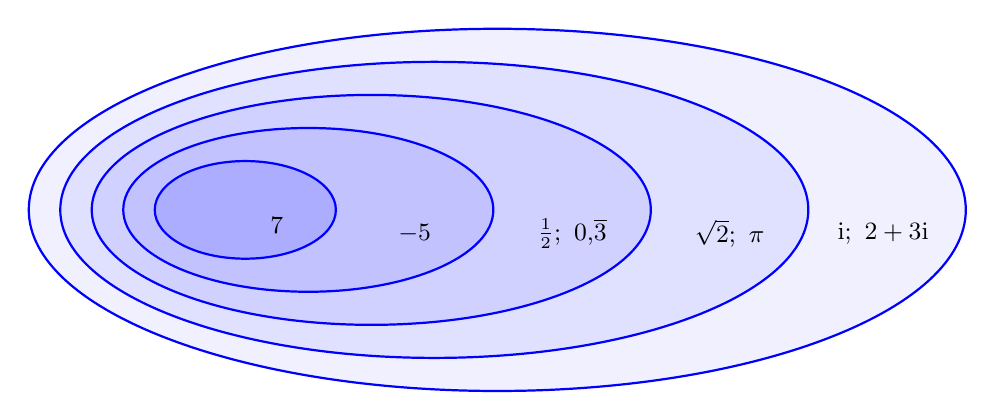
\begin{tikzpicture}[font=\small]
	\foreach \k/\col in {4/blue!6, 3/blue!12, 2/blue!18, 1/blue!24, 0/blue!32} {
		\filldraw[fill=\col, draw=blue, thick] ({0.8*\k},0) ellipse[x radius={1.15+1.2*\k}, y radius={0.62+0.42*\k}];
	}
	\node[font=\large] at (-0.35,0.2) {$\N$};       \node at (0.4,-0.2) {$7$};
	\node[font=\large] at (2.15,0.4) {$\Z$};        \node at (2.15,-0.3) {$-5$};
	\node[font=\large] at (4.15,0.4) {$\Q$};        \node at (4.15,-0.3) {$\frac12;\ 0{,}\overline{3}$};
	\node[font=\large] at (6.15,0.4) {$\R$};        \node at (6.15,-0.3) {$\sqrt2;\ \pi$};
	\node[font=\large] at (8.1,0.4) {$\C$};         \node at (8.1,-0.3) {$\mathrm{i};\ 2 + 3\mathrm{i}$};
\end{tikzpicture}
\end{center}

\begin{lesen}
\lies{$\N = \{0;\ 1;\ 2;\ \ldots\}$}{自然数|しぜんすう 全体|ぜんたい の 集合|しゅうごう}{die Menge der natürlichen Zahlen}
\lies{$\Z = \{\ldots;\ -1;\ 0;\ 1;\ \ldots\}$}{整数|せいすう 全体|ぜんたい の 集合|しゅうごう ： 正|せい の 整数|せいすう 、 負|ふ の 整数|せいすう と 0|ゼロ}{die Menge der ganzen Zahlen: positive und negative ganze Zahlen und die Null}
\lies{$\Q = \left\{\dfrac{p}{q} \;\middle|\; p, q \in \Z;\ q \neq 0\right\}$}{$p$ と $q$ が 整数|せいすう で $q$ が 0|ゼロ で ない とき 、 $q$ 分|ぶん の $p$ と 表せる|あらわせる 数|かず 全体|ぜんたい の 集合|しゅうごう}{die Menge aller Brüche $p$ durch $q$, wobei $p$ und $q$ ganze Zahlen sind und $q$ ungleich null ist}
\lies{$\R$}{実数|じっすう 全体|ぜんたい の 集合|しゅうごう ： 有限|ゆうげん 小数|しょうすう と 循環|じゅんかん 小数|しょうすう （ 有理数|ゆうりすう ） 、 および 循環|じゅんかん しない 無限|むげん 小数|しょうすう （ 無理数|むりすう ）}{die Menge der reellen Zahlen: alle abbrechenden und periodischen Dezimalbrüche (rationale Zahlen) und alle nichtabbrechenden, nichtperiodischen Dezimalbrüche (irrationale Zahlen)}
\lies{$\C = \{a + b\,\mathrm{i} \mid a, b \in \R\}$ \newline mit $\mathrm{i}^2 = -1$}{複素数|ふくそすう 全体|ぜんたい の 集合|しゅうごう ： $a$ プラス $b$ アイ 。 $a$ と $b$ は 実数|じっすう 、 アイ は 虚数|きょすう 単位|たんい}{die Menge der komplexen Zahlen: $a$ plus $b$ i, wobei $a$ und $b$ reelle Zahlen sind und i die imaginäre Einheit ist}
\lies{$\N \subset \Z \subset \Q \subset \R \subset \C$}{それぞれ の 数|かず の 集合|しゅうごう は 、 次|つぎ の 集合|しゅうごう の 真|しん 部分|ぶぶん 集合|しゅうごう で ある}{jeder Zahlbereich ist eine echte Teilmenge des nächsten}
\end{lesen}

\anmerkung{In japanischen Schulbüchern beginnen die natürlichen Zahlen (\jp{自然数}{shizensū}) bei
$1$; die Null gehört nicht dazu. Periodische Dezimalbrüche schreibt man mit Punkten über den Ziffern:
$0.\dot{3}$ statt $0{,}\overline{3}$.}

%--------------------------------------------------------------------------------------------------
\section{Mengen}

\begin{lesen}
\lies{$a \in M$}{$a$ は $M$ の 要素|ようそ で ある / $a$ は $M$ に 属する|ぞくする}{$a$ ist Element von $M$}
\lies{$a \notin M$}{$a$ は $M$ の 要素|ようそ で ない}{$a$ ist nicht Element von $M$}
\lies{$M = \{2;\ 4;\ 6\}$ \newline \footnotesize jap. $\{2,\ 4,\ 6\}$}{$M$ は 2|に 、 4|よん 、 6|ろく を 要素|ようそ と する 集合|しゅうごう}{$M$ ist die Menge mit den Elementen zwei, vier und sechs}
\lies{$M = \emptyset$}{$M$ は 空集合|くうしゅうごう で ある}{$M$ ist die leere Menge}
\lies{$A \subseteq B$}{$A$ は $B$ の 部分|ぶぶん 集合|しゅうごう で ある}{$A$ ist (eine) Teilmenge von $B$}
\lies{$A \subset B$ \newline \footnotesize jap. $A \subsetneqq B$}{$A$ は $B$ の 真|しん 部分|ぶぶん 集合|しゅうごう で ある}{$A$ ist (eine) echte Teilmenge von $B$}
\lies{$A \cup B$}{$A$ カップ $B$ / $A$ また は $B$ / $A$ と $B$ の 和集合|わしゅうごう}{$A$ vereinigt $B$ \;/\; die Vereinigungsmenge von $A$ und $B$}
\lies{$A \cap B$}{$A$ キャップ $B$ / $A$ かつ $B$ / $A$ と $B$ の 共通|きょうつう 部分|ぶぶん}{$A$ geschnitten $B$ \;/\; die Schnittmenge von $A$ und $B$}
\lies{$A \setminus B$}{$A$ と $B$ の 差集合|さしゅうごう}{$A$ ohne $B$ \;/\; die Differenzmenge von $A$ und $B$}
\lies{$A \times B$}{$A$ と $B$ の 直積|ちょくせき}{$A$ kreuz $B$ \;/\; das kartesische Produkt von $A$ und $B$}
\lies{$\{x \in \R \mid x < 4\}$}{4|よん より 小さい|ちいさい 実数|じっすう $x$ 全体|ぜんたい の 集合|しゅうごう}{die Menge aller reellen Zahlen $x$, für die gilt: $x$ ist kleiner als vier}
\end{lesen}

\anmerkung{In japanischen Schulbüchern bedeutet $A \subset B$ „Teilmenge“ einschließlich der Gleichheit.
Die Schnittmenge heißt dort \jp{共通部分}{kyōtsū bubun}, „gemeinsamer Teil“.}

%--------------------------------------------------------------------------------------------------
\section{Gleichungen und Ungleichungen lösen}

\subsection*{Beispiel: eine lineare Gleichung}

\begin{lesen}
\lies{$\dfrac{2(x - 1)}{3} + \dfrac{1}{2} = \dfrac{5}{2}$}{次|つぎ の 方程式|ほうていしき を 解きなさい|ときなさい 。}{\textit{Löse die Gleichung.}}
\lies{$4(x - 1) + 3 = 15$}{両辺|りょうへん に 分母|ぶんぼ の 最小|さいしょう 公倍数|こうばいすう 6|ろく を 掛ける|かける 。}{Multipliziere beide Seiten mit dem Hauptnenner sechs.}
\lies{$4x - 4 + 3 = 15$}{かっこ を はずす 。}{Löse die Klammern auf (multipliziere aus).}
\lies{$4x - 1 = 15$}{同類項|どうるいこう を まとめる 。}{Fasse zusammen.}
\lies{$4x = 16$}{両辺|りょうへん に 1|いち を 足す|たす 。}{Addiere eins auf beiden Seiten.}
\lies{$x = 4$}{両辺|りょうへん を $x$ の 係数|けいすう 4|よん で 割る|わる 。}{Dividiere beide Seiten durch den Koeffizienten von $x$, also durch vier.}
\lies{$L = \{4\}$}{解|かい は $x$ イコール 4|よん で ある 。}{Die Lösungsmenge enthält nur das Element vier. \;/\; Die Lösung ist $x$ gleich vier.}
\lies{\textit{Probe:} \newline $\frac{2 \cdot 3}{3} + \frac12 = \frac52$ \;\checkmark}{確かめ|たしかめ ： $x$ に 4|よん を 代入|だいにゅう する と 、 2|に 足す|たす 2|に 分|ぶん の 1|いち は 2|に 分|ぶん の 5|ご 。 \checkmark}{\textit{Probe:} Setze vier für $x$ ein: zwei plus ein Halb gleich fünf Halbe. \checkmark}
\end{lesen}

\subsection*{Beispiel: eine lineare Ungleichung}

\begin{lesen}
\lies{$3 - 2x < 9$}{次|つぎ の 不等式|ふとうしき を 解きなさい|ときなさい 。}{\textit{Löse die Ungleichung.}}
\lies{$-2x < 6$}{両辺|りょうへん から 3|さん を 引く|ひく 。}{Subtrahiere drei auf beiden Seiten.}
\lies{$x > -3$}{両辺|りょうへん を マイナス 2|に で 割る|わる 。 注意|ちゅうい ： 負|ふ の 数|かず を 掛けたり|かけたり 割ったり|わったり する と 、 不等号|ふとうごう の 向き|むき が 変わる|かわる 。}{Dividiere beide Seiten durch minus zwei. \textbf{Achtung:} Beim Multiplizieren oder Dividieren mit einer negativen Zahl dreht sich das Relationszeichen um.}
\lies{$L = \{x \in \R \mid x > -3\}$}{解|かい は 、 マイナス 3|さん より 大きい|おおきい すべて の 実数|じっすう で ある 。}{Die Lösungsmenge enthält alle reellen Zahlen, die größer als minus drei sind.}
\end{lesen}

\begin{center}
\begin{tikzpicture}[scale=0.8, font=\small]
	\draw[achse] (-6.4,0) -- (3.6,0);
	\foreach \x in {-6,...,3} {\draw (\x,0.1) -- (\x,-0.1) node[below] {$\x$};}
	\draw[blue, very thick, -{Stealth}] (-3,0) -- (3.4,0);
	\filldraw[fill=white, draw=blue, very thick] (-3,0) circle (4pt);
	\node[above, blue] at (0.2,0.15) {$x > -3$};
\end{tikzpicture}
\end{center}

\subsection*{Gleichungsarten}

\begin{lesen}
\lies{$3x - 7 = 11$}{一次|いちじ 方程式|ほうていしき ： 3|さん $x$ マイナス 7|なな イコール 11|じゅういち}{eine lineare Gleichung (Gleichung ersten Grades): drei $x$ minus sieben gleich elf}
\lies{$x^2 - 5x + 6 = 0$}{二次|にじ 方程式|ほうていしき ： $x$ 2乗|にじょう マイナス 5|ご $x$ プラス 6|ろく イコール 0|ゼロ}{eine quadratische Gleichung (Gleichung zweiten Grades): $x$ Quadrat minus fünf $x$ plus sechs gleich null}
\lies{$\sqrt{x + 3} = 5$}{無理|むり 方程式|ほうていしき ： ルート $x$ プラス 3|さん イコール 5|ご}{eine Wurzelgleichung: die Wurzel aus $x$ plus drei (aus der Summe) gleich fünf}
\lies{$2^x = 64$}{指数|しすう 方程式|ほうていしき ： 2|に の $x$ 乗|じょう イコール 64|ろくじゅうよん}{eine Exponentialgleichung: zwei hoch $x$ gleich vierundsechzig}
\lies{$\log_3 x = 4$}{対数|たいすう 方程式|ほうていしき ： ログ 3|さん の $x$ イコール 4|よん}{eine logarithmische Gleichung: Logarithmus von $x$ zur Basis drei gleich vier}
\lies{$2 \sin x = 1$}{三角|さんかく 方程式|ほうていしき ： 2|に サイン $x$ イコール 1|いち}{eine trigonometrische Gleichung: zwei mal Sinus $x$ gleich eins}
\lies{$\dfrac{x - 3}{2x + 1} = \dfrac16$}{2|に $x$ プラス 1|いち 分|ぶん の $x$ マイナス 3|さん イコール 6|ろく 分|ぶん の 1|いち}{$x$ minus drei, alles geteilt durch zwei $x$ plus eins, gleich ein Sechstel}
\end{lesen}

\anmerkung{Auch bei längeren Brüchen nennt man zuerst den ganzen Nenner, dann \textit{bun no} und den
Zähler. Klammern liest man bei Bedarf mit: \jp{かっこ}{kakko} \ldots\ \jp{かっことじ}{kakko toji}.
Arbeitsaufträge enden im Schulbuch auf \jp{なさい}{nasai}: \jp{解きなさい}{tokinasai}, „löse“.}

%--------------------------------------------------------------------------------------------------
\section{Funktionen}

\begin{lesen}
\lies{$y = f(x)$}{$y$ イコール エフ エックス / $y$ は $x$ の 関数|かんすう で ある}{$y$ gleich $f$ von $x$ \;/\; $y$ ist der Funktionswert zu $x$}
\lies{$x$}{独立|どくりつ 変数|へんすう}{die unabhängige Variable}
\lies{$y$}{従属|じゅうぞく 変数|へんすう}{die abhängige Variable}
\lies{$f\colon x \mapsto x^2$}{$f$ は $x$ に $x$ の 2乗|にじょう を 対応|たいおう させる}{$f$ ordnet $x$ das Quadrat von $x$ zu \;/\; $f$: $x$ wird abgebildet auf $x$ Quadrat}
\lies{$f(x) = 2x^2 - 3$}{エフ エックス イコール 2|に $x$ 2乗|にじょう マイナス 3|さん}{$f$ von $x$ gleich zwei $x$ Quadrat minus drei}
\lies{$f(3) = 15$}{エフ 3|さん イコール 15|じゅうご / $x$ イコール 3|さん の とき の 関数|かんすう の 値|あたい は 15|じゅうご}{$f$ von drei gleich fünfzehn \;/\; der Funktionswert an der Stelle drei ist fünfzehn}
\lies{$D_f,\ W_f$}{$f$ の 定義域|ていぎいき と 値域|ちいき}{der Definitionsbereich und der Wertebereich von $f$}
\end{lesen}

\subsection*{Der Graph einer Funktion}

\begin{center}
\begin{tikzpicture}[font=\small, scale=1.05]
	\draw[achse] (-0.7,0) -- (8.6,0) node[below left] {$x$};
	\draw[achse] (0,-1.1) -- (0,5.4) node[below left] {$y$};
	\begin{scope}
		\clip (-0.7,-1.1) rectangle (8.3,5.2);
		\draw[blue, very thick, domain=-0.35:7.75, samples=80] plot (\x, {0.1*\x*\x*\x - 1.1*\x*\x + 3.2*\x + 0.3});
	\end{scope}
	\coordinate (P) at (6.5,2.0825);
	\draw[red, thick, dashed] (P) -- (6.5,0) (P) -- (0,2.0825);
	\fill[red] (P) circle (2.5pt) node[above left] {$P(x_P \mid y_P)$};
	\node[below] at (6.5,0) {$x_P$}; \node[left] at (0,2.0825) {$y_P$};
	\node[below left] at (0,0) {$O$};
	% Beschriftungen
	\node[align=left, anchor=west] (gr) at (8.0,4.6) {$f$ のグラフ\\\color{black!60}Graph von $f$};
	\draw[-{Stealth}, thin] (gr.west) -- (7.6,4.45);
	\node[align=center] (ab) at (5.1,-1.3) {$x$ 座標\\\color{black!60}Abszisse};
	\draw[-{Stealth}, thin] (ab.east) -- (6.35,-0.35);
	\node[align=center] (or) at (-2.0,3.7) {$y$ 座標\\\color{black!60}Ordinate};
	\draw[-{Stealth}, thin] (or.south) -- (-0.15,2.55);
	\node[align=center] (ur) at (1.6,-1.3) {原点\\\color{black!60}Ursprung};
	\draw[-{Stealth}, thin] (ur.north west) -- (-0.1,-0.2);
	\node[align=center] (xa) at (8.6,0.9) {$x$ 軸\\\color{black!60}$x$-Achse};
	\node[align=center] (ya) at (1.3,5.3) {$y$ 軸\\\color{black!60}$y$-Achse};
\end{tikzpicture}
\end{center}

\begin{lesen}
\lies{$P(x_P \mid y_P)$ \newline \footnotesize jap. $P(x_P,\ y_P)$}{直交|ちょっこう 座標系|ざひょうけい で 、 座標|ざひょう が $x_P$ 、 $y_P$ の 点|てん $P$}{der Punkt $P$ mit den Koordinaten $x_P$ und $y_P$ im rechtwinkligen (kartesischen) Koordinatensystem}
\lies{$x_P$}{点|てん $P$ の $x$ 座標|ざひょう}{die Abszisse ($x$-Koordinate) von $P$}
\lies{$y_P$}{点|てん $P$ の $y$ 座標|ざひょう}{die Ordinate ($y$-Koordinate) von $P$}
\end{lesen}

\subsection*{Einteilung der elementaren Funktionen}

\begin{center}
\begin{tikzpicture}[font=\footnotesize, every node/.style={align=left, anchor=west}]
	\node (root) at (0,0)      {\jfett{初等関数}\\\color{black!60}elementare Funktionen};
	\node (alg) at (4.4,2.7)  {\jfett{代数関数}\\\color{black!60}algebraische Funktionen};
	\node (tra) at (4.4,-2.95){\jfett{超越関数}\\\color{black!60}transzendente Funktionen};
	\node (rat) at (9.2,3.7)  {有理関数\\\color{black!60}rationale Funktionen};
	\node (irr) at (9.2,1.7)  {無理関数\\\color{black!60}irrationale Funktionen\\ $y = \sqrt{x}$};
	\node (pol) at (13.0,4.75) {多項式関数\\\color{black!60}ganzrationale Funktionen\\ $y = x^3 - 2x$};
	\node (fra) at (13.0,2.75) {分数関数\\\color{black!60}gebrochenrationale F.\\ $y = \frac{x + 1}{x - 2}$};
	\node (exp) at (9.2,-0.2) {指数関数\\\color{black!60}Exponentialfunktionen\\ $y = \mathrm{e}^x$};
	\node (log) at (9.2,-2.05) {対数関数\\\color{black!60}Logarithmusfunktionen\\ $y = \ln x$};
	\node (tri) at (9.2,-3.9) {三角関数\\\color{black!60}Winkelfunktionen\\ $y = \sin x$};
	\node (arc) at (9.2,-5.75) {逆三角関数\\\color{black!60}Arkusfunktionen\\ $y = \arcsin x$};
	\foreach \a/\b in {root/alg, root/tra, alg/rat, alg/irr, rat/pol, rat/fra, tra/exp, tra/log, tra/tri, tra/arc}
		{\draw[blue, thick] (\a.east) -- ++(0.35,0) |- (\b.west);}
\end{tikzpicture}
\end{center}

\begin{lesen}
\lies{$y = \displaystyle\sum_{k=0}^{4} a_k x^k$}{$y$ イコール シグマ 、 $k$ が 0|ゼロ から 4|よん まで の $a_k$ 掛ける|かける $x$ の $k$ 乗|じょう}{$y$ gleich Summe über $a$ Index $k$ mal $x$ hoch $k$ für $k$ von null bis vier}
\lies{$y = \dfrac{7 + x}{2 - x^2}$}{$y$ イコール 2|に マイナス $x$ 2乗|にじょう 分|ぶん の 7|なな プラス $x$}{$y$ ist gleich dem Bruch mit dem Zähler sieben plus $x$ und dem Nenner zwei minus $x$ Quadrat}
\lies{$y = -\sqrt{r^2 - x^2}$}{$y$ イコール マイナス ルート $r$ 2乗|にじょう マイナス $x$ 2乗|にじょう}{$y$ gleich minus die Wurzel aus $r$ Quadrat minus $x$ Quadrat}
\lies{$y = \mathrm{e}^x$}{$y$ イコール $\mathrm{e}$ の $x$ 乗|じょう}{$y$ gleich e hoch $x$}
\lies{$y = \ln x$}{$y$ イコール ログ $x$ / $y$ は $x$ の 自然|しぜん 対数|たいすう}{$y$ gleich ln $x$ \;/\; $y$ gleich natürlicher Logarithmus von $x$}
\end{lesen}

%--------------------------------------------------------------------------------------------------
\section{Winkelfunktionen}

\begin{center}
\begin{tikzpicture}[scale=2.1, font=\small]
	\draw[achse] (-1.25,0) -- (1.5,0) node[below left] {$x$};
	\draw[achse] (0,-1.2) -- (0,1.35) node[below left] {$y$};
	\draw[blue, thick] (0,0) circle (1);
	\coordinate (P) at (35:1);
	\draw[mass] (0.3,0) arc[start angle=0, end angle=35, radius=0.3]; \node at (17:0.42) {$\alpha$};
	\draw[blue, very thick] (0,0) -- (P);
	\draw[red, very thick] (P) -- (P |- 0,0) node[midway, left, fill=white, inner sep=1pt] {$\sin\alpha$};
	\draw[green!50!black, very thick] (0,0) -- (P |- 0,0) node[midway, below] {$\cos\alpha$};
	\draw[violet, very thick] (1,0) -- (1,{tan(35)}) node[midway, right] {$\tan\alpha$};
	\draw[violet, dashed] (P) -- (1,{tan(35)});
	\fill[blue] (P) circle (1pt) node[above left] {$P$};
	\node[below] at (1,0) {$1$};
	\node[align=left, anchor=west, font=\footnotesize] at (1.55,0.9) {単位円\\\color{black!60}Einheitskreis};
\end{tikzpicture}
\end{center}

\begin{lesen}
\lies{$\sin x$}{サイン $x$ / $x$ の 正弦|せいげん}{Sinus $x$}
\lies{$\cos x$}{コサイン $x$ / $x$ の 余弦|よげん}{Kosinus $x$}
\lies{$\tan x$}{タンジェント $x$ / $x$ の 正接|せいせつ}{Tangens $x$}
\lies{$\cot x$}{コタンジェント $x$}{Kotangens $x$}
\lies{$\sec x,\ \csc x$}{セカント $x$ 、 コセカント $x$}{Sekans und Kosekans von $x$ (im deutschen Unterricht kaum verwendet)}
\lies{$\arcsin x$ \newline \footnotesize jap. meist $\sin^{-1} x$}{アークサイン $x$ / サイン インバース $x$}{Arkussinus $x$ \;/\; der Winkel, dessen Sinus $x$ ist}
\lies{$\sin 30\degree = \dfrac12$}{サイン 30|さんじゅう 度|ど は 2|に 分|ぶん の 1|いち}{der Sinus von dreißig Grad ist ein Halb}
\lies{$\tan 45\degree = 1$}{タンジェント 45|よんじゅうご 度|ど は 1|いち}{Tangens fünfundvierzig Grad gleich eins}
\lies{$\sin^2 x + \cos^2 x = 1$}{サイン 2乗|にじょう $x$ プラス コサイン 2乗|にじょう $x$ イコール 1|いち}{Sinus Quadrat $x$ plus Kosinus Quadrat $x$ gleich eins}
\lies{$5\sin^2 x - \cos 2x = 0$}{5|ご サイン 2乗|にじょう $x$ マイナス コサイン 2|に $x$ イコール 0|ゼロ}{fünf mal Sinus Quadrat $x$ minus Kosinus zwei $x$ ist gleich null}
\end{lesen}

\anmerkung{Die Winkelfunktionen heißen zusammen \jp{三角関数}{sankaku kansū}, im rechtwinkligen Dreieck
\jp{三角比}{sankakuhi}. Vorsicht bei $\sin^{-1} x$: Gemeint ist die Umkehrfunktion $\arcsin x$, nicht der
Kehrwert $\frac{1}{\sin x}$.}

%--------------------------------------------------------------------------------------------------
\section{Intervalle und Grenzwerte}

\begin{lesen}
\lies{\intervall{o}{o} \newline $]a;\,b[$ \quad jap. $(a, b)$}{$a$ から $b$ まで の 開区間|かいくかん ： $a < x < b$}{das offene Intervall von $a$ bis $b$: $a < x < b$}
\lies{\intervall{g}{g} \newline $[a;\,b]$ \quad jap. $[a, b]$}{$a$ から $b$ まで の 閉区間|へいくかん ： $a \le x \le b$}{das abgeschlossene Intervall von $a$ bis $b$: $a \le x \le b$}
\lies{\intervall{o}{g} \newline $]a;\,b]$ \quad jap. $(a, b]$}{$a$ から $b$ まで の 半開|はんかい 区間|くかん ： $a < x \le b$ （ $a$ は 含まず|ふくまず 、 $b$ は 含む|ふくむ ）}{das halboffene Intervall von $a$ bis $b$, links offen und rechts abgeschlossen: $a < x \le b$}
\lies{\intervallR \newline $[a;\,\infty[$ \quad jap. $[a, \infty)$}{$a$ 以上|いじょう の 区間|くかん ： $x \ge a$}{das Intervall von $a$ bis unendlich: $x \ge a$}
\lies{$\R = \ ]{-\infty};\,\infty[$}{実数|じっすう 全体|ぜんたい は 、 マイナス 無限大|むげんだい から プラス 無限大|むげんだい まで の 開区間|かいくかん で ある}{die Menge der reellen Zahlen ist das offene Intervall von minus unendlich bis plus unendlich}
\end{lesen}

\anmerkung{In Japan stehen runde Klammern für offene und eckige für abgeschlossene Intervalle, getrennt
durch ein Komma: $(a,\ b)$ und $[a,\ b]$. Für Monotonie-Angaben schreiben wir die Intervalle als
Ungleichungskette, z.\,B.\ \textit{fallend:} $-\infty < x \le 2$.}

\begin{lesen}
\lies{$x \to x_0$}{$x$ が $x_0$ に 近づく|ちかづく}{$x$ gegen $x$ null \;/\; $x$ strebt gegen $x$ null}
\lies{$\limxto{2} x^2 = 4$}{$x$ が 2|に に 近づく|ちかづく とき 、 $x$ 2乗|にじょう の 極限値|きょくげんち は 4|よん / リミット $x$ 矢印|やじるし 2|に の $x$ 2乗|にじょう は 4|よん}{der Grenzwert (Limes) von $x$ Quadrat für $x$ gegen zwei ist vier}
\lies{$\limxto{x_1} f(x) = L$}{$x$ が $x_1$ に 限りなく|かぎりなく 近づく|ちかづく とき 、 $f(x)$ は $L$ に 限りなく|かぎりなく 近づく|ちかづく}{Limes $f$ von $x$ für $x$ gegen $x$ eins ist groß $L$ -- $f(x)$ nähert sich $L$, wenn $x$ beliebig gegen $x_1$ strebt}
\lies{$\limxto{x_0} f(x) \neq f(x_0)$}{$x$ が $x_0$ に 近づく|ちかづく とき の $f(x)$ の 極限値|きょくげんち は $f(x_0)$ に 等しくない|ひとしくない ： 関数|かんすう $f$ は $x_0$ で 不連続|ふれんぞく で ある}{der Grenzwert von $f$ für $x$ gegen $x$ null ist ungleich $f$ von $x$ null: $f$ ist an der Stelle $x_0$ unstetig}
\lies{$\limn \dfrac{1}{n} = 0$}{$n$ を 限りなく|かぎりなく 大きく|おおきく する と 、 $n$ 分|ぶん の 1|いち は 0|ゼロ に 収束|しゅうそく する}{der Grenzwert von eins durch $n$ für $n$ gegen unendlich ist null: $\left(\frac1n\right)$ ist eine Nullfolge}
\lies{$\limn a_n = g$}{数列|すうれつ $(a_n)$ は $g$ に 収束|しゅうそく する / 極限値|きょくげんち は $g$ で ある}{die Folge $(a_n)$ konvergiert gegen $g$ \;/\; sie ist konvergent mit dem Grenzwert $g$}
\end{lesen}

%--------------------------------------------------------------------------------------------------
\section{Differenzialrechnung}

\begin{center}
\begin{tikzpicture}[scale=1.25, font=\small]
	\draw[achse] (-0.4,0) -- (5,0) node[below left] {$x$};
	\draw[achse] (0,-0.4) -- (0,4.4) node[below left] {$y$};
	\begin{scope}
		\clip (-0.4,-0.4) rectangle (4.8,4.2);
		\draw[blue, very thick, domain=0:4.6, samples=60] plot (\x, {0.2*\x*\x + 0.4});
		% Sekante durch P(1|0,6) und Q(3,5|2,85), Steigung 0,9
		\draw[red, thick, dashed, domain=0:4.8] plot (\x, {0.9*(\x-1) + 0.6});
		% Tangente in P, Steigung 0,4
		\draw[red, very thick, domain=0:4.8] plot (\x, {0.4*(\x-1) + 0.6});
	\end{scope}
	\fill (1,0.6) circle (2pt) node[above left] {$P$};
	\fill (3.5,2.85) circle (2pt) node[above left] {$Q$};
	\draw[black!60] (1,0.6) -- node[below] {$h = \Delta x$} (3.5,0.6) -- node[right] {$\Delta y$} (3.5,2.85);
	\draw[black!40, dotted] (1,0.6) -- (1,0) node[below, black] {$x_0$};
	\draw[black!40, dotted] (3.5,0.6) -- (3.5,0) node[below, black] {$x_0 + h$};
	\node[red, align=left, anchor=west] at (4.85,3.8) {割線 -- Sekante};
	\node[red, align=left, anchor=west] at (4.85,2.2) {接線 -- Tangente};
\end{tikzpicture}
\end{center}

\begin{lesen}
\lies{$\dfrac{f(x_0 + h) - f(x_0)}{h}$}{平均|へいきん 変化率|へんかりつ ： 2点|にてん $P$ 、 $Q$ を 通る|とおる 直線|ちょくせん の 傾き|かたむき}{der Differenzenquotient: die Steigung der Sekante durch $P$ und $Q$}
\lies{$f'(x_0) = {}$ \newline $\displaystyle\lim_{h \to 0} \frac{f(x_0 + h) - f(x_0)}{h}$}{エフ ダッシュ $x_0$ は 、 $h$ が 0|ゼロ に 近づく|ちかづく とき の 平均|へいきん 変化率|へんかりつ の 極限値|きょくげんち 。 図形的|ずけいてき に は 、 点|てん $P$ に おける 接線|せっせん の 傾き|かたむき で ある 。}{$f$ Strich von $x$ null ist der Grenzwert für $h$ gegen null von $f$ von $x$ null plus $h$ minus $f$ von $x$ null, alles durch $h$. Geometrisch ist das die Steigung der Tangente in $P$.}
\lies{$f'(x),\ f''(x),\ f^{(n)}(x)$}{第|だい 1|いち 次|じ 、 第|だい 2|に 次|じ 、 第|だい $n$ 次|じ 導関数|どうかんすう ： エフ ダッシュ エックス 、 エフ ツー ダッシュ エックス 、 エフ エヌ エックス}{die erste, zweite, $n$-te Ableitung von $f$: $f$ Strich von $x$, $f$ zwei Strich von $x$, $f$ $n$ Strich von $x$}
\lies{$\dfrac{\mathrm{d}y}{\mathrm{d}x}$}{ディー ワイ ディー エックス ： $y$ を $x$ で 微分|びぶん した もの}{d $y$ nach d $x$ -- der Differenzialquotient von $y$}
\lies{$\dfrac{\mathrm{d}^2 y}{\mathrm{d}x^2}$}{ディー 2乗|にじょう ワイ ディー エックス 2乗|にじょう}{d zwei $y$ nach d $x$ Quadrat}
\lies{$\dfrac{\mathrm{d}^n y}{\mathrm{d}x^n}$}{ディー $n$ 乗|じょう ワイ ディー エックス $n$ 乗|じょう}{d $n$ $y$ nach d $x$ hoch $n$}
\lies{$\dfrac{\partial z}{\partial x}$}{ラウンド ディー ゼット ラウンド ディー エックス ： $z$ の $x$ に 関する|かんする 偏導関数|へんどうかんすう}{d $z$ partiell nach d $x$}
\lies{$\dot{s} = \dfrac{\mathrm{d}s}{\mathrm{d}t}$}{エス ドット イコール ディー エス ディー ティー （ 時間|じかん に 関する|かんする 微分|びぶん ）}{$s$ Punkt gleich d $s$ nach d $t$ (Ableitung nach der Zeit)}
\end{lesen}

\subsection*{Beispiele}

\begin{lesen}
\lies{$(x^3)' = 3x^2$}{$x$ 3乗|さんじょう の 導関数|どうかんすう は 3|さん $x$ 2乗|にじょう}{die Ableitung von $x$ hoch drei ist drei $x$ Quadrat}
\lies{$(\sin x)' = \cos x$}{サイン $x$ を 微分|びぶん する と コサイン $x$}{die (erste) Ableitung von Sinus $x$ ist Kosinus $x$}
\lies{$f(x) = x^2 - 4x$ \newline $f'(x) = 2x - 4$}{$f(x)$ を 微分|びぶん する ： エフ ダッシュ エックス イコール 2|に $x$ マイナス 4|よん 。}{Leite $f$ ab: $f$ Strich von $x$ gleich zwei $x$ minus vier.}
\lies{$2x - 4 = 0 \ \Rightarrow\ x_E = 2$}{導関数|どうかんすう を 0|ゼロ と おいて 、 $x$ に ついて 解く|とく 。}{Setze die erste Ableitung gleich null und löse nach $x$ auf.}
\lies{$f''(2) = 2 > 0$}{$x$ イコール 2|に で の 第|だい 2|に 次|じ 導関数|どうかんすう の 値|あたい は 正|せい な の で 、 グラフ は そこ で 極小|きょくしょう と なる ： $T(2,\,-4)$}{Die zweite Ableitung an der Stelle zwei ist positiv, also hat der Graph dort einen Tiefpunkt: $T(2 \mid -4)$.}
\end{lesen}

%--------------------------------------------------------------------------------------------------
\section{Integralrechnung}

\begin{center}
\begin{tikzpicture}[scale=1.15, font=\small]
	% Untersumme (grau) und Obersumme (rot gestrichelt) für f(x) = 0,15x^2 + 0,6 auf [1; 5], n = 8
	\foreach \i in {0,...,7} {
		\pgfmathsetmacro{\xl}{1+0.5*\i} \pgfmathsetmacro{\xr}{1.5+0.5*\i}
		\pgfmathsetmacro{\yl}{0.15*\xl*\xl+0.6} \pgfmathsetmacro{\yr}{0.15*\xr*\xr+0.6}
		\filldraw[fill=gray!35, draw=gray] (\xl,0) rectangle (\xr,\yl);
		\draw[red, dashed] (\xl,\yl) -- (\xl,\yr) -- (\xr,\yr) -- (\xr,\yl);
	}
	\draw[achse] (-0.4,0) -- (6.2,0) node[below left] {$x$};
	\draw[achse] (0,-0.4) -- (0,5) node[below left] {$y$};
	\draw[blue, very thick, domain=0:5.6, samples=60] plot (\x, {0.15*\x*\x + 0.6}) node[right] {$f$};
	\draw[black!60] (1,0) -- (1,0.75); \draw[black!60] (5,0) -- (5,4.35);
	\node[below] at (1,0) {$a$}; \node[below] at (5,0) {$b$};
	\draw[|<->|, black!70] (3,-0.5) -- node[below] {$\Delta x$} (3.5,-0.5);
	\node[align=left, anchor=west] at (6.4,1.2) {\textcolor{gray}{\rule{8pt}{8pt}} 不足和 -- Untersumme\\[2pt] \textcolor{red}{\rule[2pt]{8pt}{0.8pt}} 過剰和 -- Obersumme};
\end{tikzpicture}
\end{center}

\begin{lesen}
\lies{$\displaystyle\int f(x)\dx = F(x) + C$, \newline wenn $F'(x) = f(x)$}{$F'(x)$ が $f(x)$ に 等しい|ひとしい とき 、 インテグラル エフ エックス ディー エックス は 、 ラージ エフ エックス プラス $C$}{Integral $f$ von $x$ d $x$ ist gleich groß $F$ von $x$ plus groß $C$, wenn groß $F$ Strich von $x$ gleich $f$ von $x$ ist}
\lies{$\displaystyle\int f(x)\dx$}{$f$ の 不定|ふてい 積分|せきぶん 。 $F$ は $f$ の 原始|げんし 関数|かんすう 、 $C$ は 積分|せきぶん 定数|ていすう}{das unbestimmte Integral von $f$; $F$ ist eine Stammfunktion von $f$, $C$ die Integrationskonstante}
\lies{$\displaystyle\int_a^b f(x)\dx$}{インテグラル $a$ から $b$ まで エフ エックス ディー エックス ： 下端|かたん $a$ 、 上端|じょうたん $b$ の 定積分|ていせきぶん}{Integral von $a$ bis $b$ über $f$ von $x$ d $x$ -- ein bestimmtes Integral mit der unteren Grenze $a$ und der oberen Grenze $b$}
\lies{$\big[F(x)\big]_a^b = F(b) - F(a)$}{$F(x)$ に $b$ を 代入|だいにゅう した 値|あたい から 、 $a$ を 代入|だいにゅう した 値|あたい を 引く|ひく}{groß $F$ von $x$ in den Grenzen von $a$ bis $b$ ist gleich $F$ von $b$ minus $F$ von $a$}
\lies{$\displaystyle\lim_{\Delta x \to 0} \sum_{k} f(x_k)\,\Delta x$}{デルタ $x$ を 0|ゼロ に 近づけた|ちかづけた とき の 、 $f(x_k)$ 掛ける|かける デルタ $x$ の 和|わ の 極限値|きょくげんち}{der Grenzwert für Delta $x$ gegen null der Summe über $f$ von $x$ Index $k$ mal Delta $x$}
\lies{$\displaystyle\int_a^b f(x)\dx = A$}{$f(x) \ge 0$ の とき ： $f$ の グラフ 、 $x$ 軸|じく 、 直線|ちょくせん $x = a$ と $x = b$ で 囲まれた|かこまれた 部分|ぶぶん の 面積|めんせき}{für $f(x) \ge 0$: der Inhalt der Fläche zwischen dem Graphen von $f$, der $x$-Achse und den Geraden $x = a$ und $x = b$}
\end{lesen}

\subsection*{Beispiele}

\begin{lesen}
\lies{$\displaystyle\int \cos x \dx = \sin x + C$}{インテグラル コサイン $x$ ディー エックス イコール サイン $x$ プラス $C$}{Integral Kosinus $x$ d $x$ gleich Sinus $x$ plus $C$}
\lies{$\displaystyle\int_0^2 x^2 \dx = \left[\tfrac13 x^3\right]_0^2 = \tfrac83$}{$x$ 2乗|にじょう を 0|ゼロ から 2|に まで 積分|せきぶん する と 、 3|さん 分|ぶん の 8|はち}{Integral von null bis zwei über $x$ Quadrat d $x$ gleich ein Drittel $x$ hoch drei in den Grenzen von null bis zwei, also acht Drittel}
\lies{$\displaystyle\int_1^{\mathrm{e}} \frac{1}{x} \dx = \big[\ln x\big]_1^{\mathrm{e}} = 1$}{$x$ 分|ぶん の 1|いち を 1|いち から $\mathrm{e}$ まで 積分|せきぶん する と 、 1|いち}{Integral von eins bis e über eins durch $x$ d $x$ gleich ln $x$ in den Grenzen von eins bis e, also eins}
\end{lesen}

\anmerkung{Wichtige Anwendungen der Integralrechnung in der Geometrie: Flächeninhalte
(\jp{面積}{menseki}), Volumina (\jp{体積}{taiseki}) und Bogenlängen (\jp{弧の長さ}{ko no nagasa}).
Das Integralzeichen liest man \jp{インテグラル}{integuraru}, den Strich der Ableitung \jp{ダッシュ}{dasshu}.}

%--------------------------------------------------------------------------------------------------
\section{Geraden und Winkel}

\begin{center}
\begin{tikzpicture}[font=\small]
	\draw[mass] (1.3,0) arc[start angle=0, end angle=40, radius=1.3]; \node at (20:0.9) {$\alpha$};
	\draw[blue, very thick] (4.6,0) -- (0,0) -- (40:4.6);
	\fill (0,0) circle (2pt) node[above left] {$S$}; \fill (3.2,0) circle (2pt) node[below] {$A$}; \fill (40:3.2) circle (2pt) node[above left] {$B$};
	\node[align=center] (v) at (-2.2,-0.9) {頂点\\\color{black!60}Scheitel};
	\draw[-{Stealth}, thin] (v.east) -- (-0.15,-0.1);
	\node[align=center] (l) at (6.6,0.9) {辺\\\color{black!60}Schenkel};
	\draw[-{Stealth}, thin] (l.west) -- (4.3,0.1); \draw[-{Stealth}, thin] (l.west) -- ($(40:4.3)+(0.15,-0.1)$);
\end{tikzpicture}
\end{center}

\begin{lesen}
\lies{$g$}{直線|ちょくせん $g$}{die Gerade $g$}
\lies{$\overline{AB}$}{線分|せんぶん $AB$ / $A$ から $B$ まで の 距離|きょり}{die Strecke $A$ $B$}
\lies{$g \parallel h$ \newline \footnotesize jap. $g \mathbin{/\!/} h$}{$g$ 平行|へいこう $h$ / $g$ は $h$ に 平行|へいこう で ある}{$g$ ist parallel zu $h$}
\lies{$g \perp h$}{$g$ 垂直|すいちょく $h$ / $g$ は $h$ に 垂直|すいちょく で ある}{$g$ ist senkrecht zu $h$ \;/\; $g$ steht senkrecht auf $h$}
\lies{$\sphericalangle ASB$ \newline \footnotesize jap. $\angle ASB$}{角|かく $ASB$ （ 頂点|ちょうてん を 真ん中|まんなか に 書く|かく ）}{Winkel $A$ $S$ $B$ (der Scheitel steht in der Mitte)}
\lies{$\alpha = 40\degree$}{アルファ は 40|よんじゅう 度|ど ： 鋭角|えいかく}{Alpha gleich vierzig Grad: ein spitzer Winkel}
\lies{$\alpha + \beta = 90\degree$}{アルファ と ベータ は 互い|たがい に 余角|よかく ： 和|わ が 90|きゅうじゅう 度|ど}{Alpha und Beta sind Komplementwinkel: Sie ergänzen sich zu neunzig Grad}
\lies{$\alpha + \beta = 180\degree$}{アルファ と ベータ は 互い|たがい に 補角|ほかく ： 和|わ が 180|ひゃくはちじゅう 度|ど}{Alpha und Beta sind Supplementwinkel: Sie ergänzen sich zu hundertachtzig Grad}
\end{lesen}

\subsection*{Winkel an geschnittenen Parallelen}

\begin{center}
\begin{tikzpicture}[font=\small, scale=1.1]
	\coordinate (S1) at (0.6,2.2); \coordinate (S2) at (-0.67,0);
	\draw[red, thin] (S1) circle (0.42); \draw[red, thin] (S2) circle (0.42);
	\draw[blue, very thick] (-4,2.2) -- (4,2.2) node[right] {$g_1$};
	\draw[blue, very thick] (-4,0) -- (4,0) node[right] {$g_2$};
	\draw[blue, very thick] ($(S2)+(240:1.5)$) -- ($(S1)+(60:1.5)$) node[right] {$t$};
	\foreach \w/\n in {30/\alpha, 120/\beta, 210/\gamma, 300/\delta} {
		\node at ($(S1)+(\w:0.78)$) {$\n_1$}; \node at ($(S2)+(\w:0.78)$) {$\n_2$};}
	\node[align=left, anchor=west] at (5,1.1) {$g_1 \parallel g_2$\\ $t$: 2直線に交わる直線\\\color{black!60}Transversale (schneidende Gerade)};
\end{tikzpicture}
\end{center}

\begin{lesen}
\lies{$\alpha_1$ und $\alpha_2$}{同位角|どういかく ： 2直線|にちょくせん が 平行|へいこう ならば 等しい|ひとしい}{Stufenwinkel -- an Parallelen gleich groß}
\lies{$\gamma_1$ und $\alpha_2$}{錯角|さっかく ： 2直線|にちょくせん が 平行|へいこう ならば 等しい|ひとしい}{Wechselwinkel -- an Parallelen gleich groß}
\lies{$\delta_1$ und $\alpha_2$}{同側|どうそく 内角|ないかく ： 2直線|にちょくせん が 平行|へいこう ならば 、 和|わ は $180\degree$}{entgegengesetzt liegende Winkel -- ergänzen sich an Parallelen zu $180\degree$}
\lies{$\alpha_1$ und $\gamma_1$}{対頂角|たいちょうかく ： 常|つね に 等しい|ひとしい}{Scheitelwinkel -- immer gleich groß}
\lies{$\alpha_1$ und $\beta_1$}{隣接|りんせつ 補角|ほかく ： 和|わ は $180\degree$}{Nebenwinkel -- ergänzen sich zu $180\degree$}
\end{lesen}

\subsection*{Beispiele}

\begin{lesen}
\lies{$\alpha_1 = 65\degree$ \newline $\beta_1 = 180\degree - 65\degree = 115\degree$}{アルファ 1|いち は 65|ろくじゅうご 度|ど 。 ベータ 1|いち は その 隣接|りんせつ 補角|ほかく な の で 、 115|ひゃくじゅうご 度|ど 。}{Alpha eins beträgt fünfundsechzig Grad. Beta eins ist der Nebenwinkel, also hundertfünfzehn Grad.}
\lies{$\gamma_1 = \alpha_1 = 65\degree$}{ガンマ 1|いち と アルファ 1|いち は 対頂角|たいちょうかく な の で 等しい|ひとしい 。}{Gamma eins und Alpha eins sind Scheitelwinkel, also gleich groß.}
\lies{$\alpha_2 = \alpha_1 = 65\degree$}{アルファ 2|に と アルファ 1|いち は 平行線|へいこうせん の 同位角|どういかく な の で 等しい|ひとしい 。}{Alpha zwei und Alpha eins sind Stufenwinkel an Parallelen, also gleich groß.}
\lies{$\alpha = 90\degree$}{直線|ちょくせん $g$ と $h$ は 垂直|すいちょく に 交わる|まじわる 。}{Die Geraden $g$ und $h$ schneiden einander rechtwinklig.}
\end{lesen}

%--------------------------------------------------------------------------------------------------
\section{Dreiecke, Vierecke und Vielecke}

\begin{center}
\begin{tikzpicture}[font=\small, scale=1.1]
	\draw[mass] (0.7,0) arc[start angle=0, end angle=59.04, radius=0.7]; \node at (28:0.45) {$\alpha$};
	\draw[mass] ($(5,0)+(136.85:0.7)$) arc[start angle=136.85, end angle=180, radius=0.7]; \node at ($(5,0)+(160:1.0)$) {$\beta$};
	\draw[mass] ($(1.8,3)+(239.04:0.6)$) arc[start angle=239.04, end angle=316.85, radius=0.6]; \node at ($(1.8,3)+(280:0.9)$) {$\gamma$};
	\draw[mass] (5.9,0) arc[start angle=0, end angle=136.85, radius=0.9]; \node at ($(5,0)+(60:1.2)$) {$\delta$};
	\draw[black!60, thick, dashed] (1.8,3) -- node[right, pos=0.6] {$h_c$} (1.8,0);
	\draw[black!60, thick] (2.15,0) arc[start angle=0, end angle=90, radius=0.35]; \fill[black!60] (1.95,0.15) circle (0.8pt);
	\draw[blue, very thick] (0,0) -- node[below] {$c$} (5,0) -- node[above right] {$a$} (1.8,3) -- node[above left] {$b$} cycle;
	\draw[blue, thick, dashed] (5,0) -- (6.6,0);
	\node[below left] at (0,0) {$A$}; \node[below] at (5,0) {$B$}; \node[above] at (1.8,3) {$C$};
	\node[align=left, anchor=west] at (7.4,2.2) {$a,\ b,\ c$: 辺 -- \color{black!60}Seiten};
	\node[align=left, anchor=west] at (7.4,1.6) {$\alpha,\ \beta,\ \gamma$: 内角 -- \color{black!60}Innenwinkel};
	\node[align=left, anchor=west] at (7.4,1.0) {$\delta$: 外角 -- \color{black!60}Außenwinkel};
	\node[align=left, anchor=west] at (7.4,0.4) {$h_c$: 高さ -- \color{black!60}Höhe};
\end{tikzpicture}
\end{center}

\begin{lesen}
\lies{$\triangle ABC$}{三角形|さんかくけい $ABC$}{Dreieck $A$ $B$ $C$}
\lies{$\alpha + \beta + \gamma = 180\degree$}{三角形|さんかくけい の 内角|ないかく の 和|わ は 180|ひゃくはちじゅう 度|ど}{die Innenwinkel eines Dreiecks ergeben zusammen hundertachtzig Grad}
\lies{$\delta = \alpha + \gamma$}{外角|がいかく は 、 それ と 隣り合わない|となりあわない 2つ|ふたつ の 内角|ないかく の 和|わ に 等しい|ひとしい}{ein Außenwinkel ist so groß wie die beiden nicht anliegenden Innenwinkel zusammen}
\lies{$A = \dfrac{1}{2} \cdot c \cdot h_c$}{面積|めんせき は 、 底辺|ていへん 掛ける|かける 高さ|たかさ 割る|わる 2|に}{der Flächeninhalt ist gleich ein Halb mal Grundseite mal Höhe}
\lies{$a^2 + b^2 = c^2$}{$a$ 2乗|にじょう プラス $b$ 2乗|にじょう イコール $c$ 2乗|にじょう 。 三平方|さんへいほう の 定理|ていり ： 直角|ちょっかく 三角形|さんかくけい で は 、 斜辺|しゃへん の 2乗|にじょう は 、 他|ほか の 2辺|にへん の 2乗|にじょう の 和|わ に 等しい|ひとしい}{$a$ Quadrat plus $b$ Quadrat gleich $c$ Quadrat -- Satz des Pythagoras: Im rechtwinkligen Dreieck ist das Hypotenusenquadrat so groß wie die beiden Kathetenquadrate zusammen}
\lies{$\triangle ABC \cong \triangle DEF$ \newline \footnotesize jap. $\triangle ABC \equiv \triangle DEF$}{三角形|さんかくけい $ABC$ と 三角形|さんかくけい $DEF$ は 合同|ごうどう で ある}{Dreieck $A$ $B$ $C$ ist kongruent zu Dreieck $D$ $E$ $F$}
\lies{$\triangle ABC \sim \triangle PQR$ \newline \footnotesize jap. $\triangle ABC \backsim \triangle PQR$}{三角形|さんかくけい $ABC$ と 三角形|さんかくけい $PQR$ は 相似|そうじ で ある}{Dreieck $A$ $B$ $C$ ist ähnlich zu Dreieck $P$ $Q$ $R$}
\end{lesen}

\subsection*{Besondere Dreiecke}

\begin{lesen}
\lies{\skGleichschenklig}{二等辺|にとうへん 三角形|さんかくけい ： 2辺|にへん が 等しい|ひとしい 。 残り|のこり の 辺|へん が 底辺|ていへん で 、 2つ|ふたつ の 底角|ていかく は 等しい|ひとしい}{ein gleichschenkliges Dreieck: zwei gleich lange Seiten (Schenkel), die dritte Seite ist die Basis; die Basiswinkel sind gleich groß}
\lies{\skRechtwinklig}{直角|ちょっかく 三角形|さんかくけい ： 直角|ちょっかく に 向かい合う|むかいあう 辺|へん が 斜辺|しゃへん}{ein rechtwinkliges Dreieck: Die Katheten schließen den rechten Winkel ein, die Hypotenuse liegt ihm gegenüber}
\end{lesen}

\begin{center}
\begin{tikzpicture}[font=\small, scale=1.0]
	\coordinate (A) at (0,0); \coordinate (B) at (3.6,0); \coordinate (C) at (1.8,3.118); \coordinate (M) at (1.8,1.039);
	\draw[red, thick] (M) circle (1.039); \draw[red, thick] (M) circle (2.078);
	\foreach \p/\q in {A/{2.7,1.559}, B/{0.9,1.559}, C/{1.8,0}} {\draw[black!60, dash dot] ($(\p)!-0.25!(\q)$) -- ($(\p)!1.45!(\q)$);}
	\draw[blue, very thick] (A) -- (B) -- (C) -- cycle; \fill (M) circle (2pt) node[right=2pt] {$M$};
	\node[align=left, anchor=west] at (5.2,3.1) {正三角形と3本の対称の軸\\\color{black!60}ein gleichseitiges Dreieck mit seinen drei Symmetrieachsen};
	\node[align=left, anchor=west] at (5.2,1.9) {\textcolor{red}{内接円}と\textcolor{red}{外接円} --
		\color{black!60}Inkreis und Umkreis};
	\node[align=left, anchor=west, text width=10cm] at (5.2,0.2) {点 $M$ は、垂線、垂直二等分線、中線、角の二等分線の交点である。\\\color{black!60}$M$ ist der Schnittpunkt der Höhen, der Mittelsenkrechten, der Seitenhalbierenden und der Winkelhalbierenden.};
\end{tikzpicture}
\end{center}

\subsection*{Vierecke und regelmäßige Vielecke}

\begin{lesen}
\lies{\skTrapez}{台形|だいけい ： 1組|ひとくみ の 向かい合う|むかいあう 辺|へん が 平行|へいこう な 四角形|しかくけい}{ein Trapez: ein Viereck mit einem Paar paralleler Seiten}
\lies{\skParallelogramm}{平行|へいこう 四辺形|しへんけい ： 2組|ふたくみ の 向かい合う|むかいあう 辺|へん が それぞれ 平行|へいこう な 四角形|しかくけい}{ein Parallelogramm: ein Viereck, dessen gegenüberliegende Seiten parallel sind}
\lies{\skRaute}{ひし形|ひしがた ： 4つ|よっつ の 辺|へん が すべて 等しい|ひとしい 四角形|しかくけい}{eine Raute (ein Rhombus): ein Parallelogramm mit vier gleich langen Seiten}
\lies{\skRechteck}{長方形|ちょうほうけい ： 4つ|よっつ の 角|かく が すべて 直角|ちょっかく の 四角形|しかくけい}{ein Rechteck: ein Viereck mit vier rechten Winkeln}
\lies{\skQuadrat}{正方形|せいほうけい ： 4つ|よっつ の 辺|へん が すべて 等しい|ひとしい 長方形|ちょうほうけい}{ein Quadrat: ein Rechteck mit vier gleich langen Seiten}
\lies{\skNeck{5} \skNeck{6} \skNeck{8}}{正多角形|せいたかくけい ： 正五角形|せいごかくけい 、 正六角形|せいろっかくけい 、 正八角形|せいはっかくけい （ 辺|へん も 角|かく も すべて 等しい|ひとしい ）}{regelmäßige Vielecke: ein Fünfeck, ein Sechseck und ein Achteck (alle Seiten und alle Winkel sind gleich groß)}
\end{lesen}

\subsection*{Beispiele}

\begin{lesen}
\lies{$a = 3\,\mathrm{cm},\ b = 4\,\mathrm{cm}$ \newline $c = \sqrt{3^2 + 4^2}\,\mathrm{cm} = 5\,\mathrm{cm}$}{直角|ちょっかく を はさむ 2辺|にへん が 3|さん センチメートル と 4|よん センチメートル の 直角|ちょっかく 三角形|さんかくけい で は 、 斜辺|しゃへん は ルート 3|さん の 2乗|にじょう プラス 4|よん の 2乗|にじょう で 、 5|ご センチメートル 。}{In einem rechtwinkligen Dreieck sind die Katheten drei und vier Zentimeter lang. Die Hypotenuse ist die Wurzel aus drei Quadrat plus vier Quadrat, also fünf Zentimeter.}
\lies{$A = \frac12 \cdot 8\,\mathrm{cm} \cdot 5\,\mathrm{cm} = 20\,\mathrm{cm}^2$}{三角形|さんかくけい の 面積|めんせき は 、 8|はち センチメートル 掛ける|かける 5|ご センチメートル 割る|わる 2|に で 、 20|にじゅう 平方|へいほう センチメートル 。}{Der Flächeninhalt des Dreiecks ist ein Halb mal acht Zentimeter mal fünf Zentimeter, also zwanzig Quadratzentimeter.}
\lies{$u = 2 \cdot 6\,\mathrm{cm} + 2 \cdot 4\,\mathrm{cm} = 20\,\mathrm{cm}$}{縦|たて 4|よん センチメートル 、 横|よこ 6|ろく センチメートル の 長方形|ちょうほうけい の 周|しゅう の 長さ|ながさ は 、 20|にじゅう センチメートル 。}{Der Umfang eines Rechtecks mit sechs Zentimetern Länge und vier Zentimetern Breite beträgt zwanzig Zentimeter.}
\lies{$(6 - 2) \cdot 180\degree = 720\degree$}{六角形|ろっかくけい の 内角|ないかく の 和|わ は 720|ななひゃくにじゅう 度|ど 。}{Die Innenwinkel eines Sechsecks ergeben zusammen siebenhundertzwanzig Grad.}
\end{lesen}

%--------------------------------------------------------------------------------------------------
\section{Der Kreis und seine Teile}

\begin{center}
\begin{tikzpicture}[font=\small, scale=1.2]
	\fill[gray!40] (120:2) arc[start angle=120, end angle=200, radius=2] -- cycle;
	\fill[blue!15] (0,0) -- (300:2) arc[start angle=300, end angle=345, radius=2] -- cycle;
	\draw[blue, very thick] (0,0) circle (2);
	\draw[blue, thick] (120:2) -- node[right, black, inner sep=2pt, pos=0.2] {$s$} (200:2);
	\draw[blue, thick] (300:2) -- (0,0) -- (345:2);
	\draw[black!70, thick] (90:2) -- node[left, pos=0.75] {$d$} (270:2);
	\draw[black!70, thick] (0,0) -- node[above] {$r$} (15:2);
	\draw[red, line width=2pt] (35:2) arc[start angle=35, end angle=75, radius=2]; \node[red] at (55:2.3) {$b$};
	\draw[red, thick] (-2.7,2) -- (2.7,2) node[right] {$t$};
	\fill[red] (0,2) circle (2pt) node[above] {$B$};
	\draw[red, thick] ($(215:2)!-0.5!(255:2)$) -- ($(215:2)!1.6!(255:2)$) node[right] {$g$};
	\fill (0,0) circle (2pt) node[left] {$M$};
	\node at (160:1.75) {$A_1$}; \node at (322:1.3) {$A_2$};
\end{tikzpicture}
\end{center}

\begin{lesen}
\lies{$M$}{中心|ちゅうしん}{der Mittelpunkt}
\lies{$r$}{半径|はんけい}{der Radius -- Plural: Radien}
\lies{$d = 2r$}{直径|ちょっけい ： 直径|ちょっけい は 半径|はんけい の 2倍|にばい}{der Durchmesser: Er ist doppelt so groß wie der Radius}
\lies{$s$}{弦|げん ： 円周上|えんしゅうじょう の 2点|にてん を 結ぶ|むすぶ 線分|せんぶん}{eine Sehne: eine Strecke zwischen zwei Punkten des Kreises}
\lies{$g$}{割線|かっせん ： 円|えん と 2点|にてん で 交わる|まじわる 直線|ちょくせん}{eine Sekante: eine Gerade, die den Kreis in zwei Punkten schneidet}
\lies{$t$, $B$}{接線|せっせん ： 円|えん と 1点|いってん （ 接点|せってん $B$ ） だけ を 共有|きょうゆう する 直線|ちょくせん 。 接線|せっせん は 、 接点|せってん を 通る|とおる 半径|はんけい に 垂直|すいちょく}{eine Tangente: eine Gerade, die den Kreis in einem Punkt berührt, dem Berührungspunkt $B$; sie steht senkrecht auf dem Berührungsradius}
\lies{$b$}{弧|こ}{ein Kreisbogen}
\lies{$A_1$}{弓形|きゅうけい ： 弦|げん と 弧|こ で 囲まれた|かこまれた 部分|ぶぶん}{ein Kreisabschnitt (Kreissegment): die Fläche zwischen Sehne und Bogen}
\lies{$A_2$}{扇形|おうぎがた ： 2本|にほん の 半径|はんけい と 弧|こ で 囲まれた|かこまれた 部分|ぶぶん}{ein Kreisausschnitt (Kreissektor): die Fläche zwischen zwei Radien und einem Bogen}
\lies{$u = 2\pi r$}{円周|えんしゅう は 2|に パイ $r$}{der Umfang ist gleich zwei pi $r$}
\lies{$A = \pi r^2$}{面積|めんせき は パイ $r$ 2乗|にじょう}{der Flächeninhalt ist gleich pi $r$ Quadrat}
\end{lesen}

\subsection*{Beispiele}

\begin{lesen}
\lies{$r = 5\,\mathrm{cm}$ \newline $u = 2\pi \cdot 5\,\mathrm{cm} \approx 31{,}4\,\mathrm{cm}$}{半径|はんけい が 5|ご センチメートル な の で 、 円周|えんしゅう は 2|に パイ 掛ける|かける 5|ご センチメートル で 、 約|やく 31.4|さんじゅういってん_よん センチメートル 。}{Der Radius beträgt fünf Zentimeter, also ist der Umfang zwei pi mal fünf Zentimeter, ungefähr einunddreißig Komma vier Zentimeter.}
\lies{$A = \pi \cdot (5\,\mathrm{cm})^2 \approx 78{,}5\,\mathrm{cm}^2$}{面積|めんせき は パイ 掛ける|かける 5|ご センチメートル の 2乗|にじょう で 、 約|やく 78.5|ななじゅうはってん_ご 平方|へいほう センチメートル 。}{Der Flächeninhalt ist pi mal fünf Zentimeter zum Quadrat, ungefähr achtundsiebzig Komma fünf Quadratzentimeter.}
\lies{$b = \dfrac{60\degree}{360\degree} \cdot 2\pi \cdot 5\,\mathrm{cm} \approx 5{,}24\,\mathrm{cm}$}{中心角|ちゅうしんかく 60|ろくじゅう 度|ど に 対する|たいする 弧|こ は 円周|えんしゅう の 6|ろく 分|ぶん の 1|いち で 、 約|やく 5.24|ご_てん_に_よん センチメートル 。}{Der Bogen zu einem Winkel von sechzig Grad ist ein Sechstel des Umfangs, etwa fünf Komma zwei vier Zentimeter.}
\end{lesen}

%--------------------------------------------------------------------------------------------------
\section{Körper berechnen}

\begin{center}
\begin{tikzpicture}[font=\small]
	\def\dx{1.2}\def\dy{0.9}
	\draw[blue, thick, dashed] (0,0) -- (\dx,\dy) -- (4+\dx,\dy) (\dx,\dy) -- (\dx,2.5+\dy);
	\draw[red, thick, dashed] (0,0) -- (4+\dx,\dy);
	\draw[red, very thick] (0,0) -- (4+\dx,2.5+\dy);
	\draw[blue, very thick] (0,0) rectangle (4,2.5) (4,0) -- (4+\dx,\dy) -- (4+\dx,2.5+\dy) -- (\dx,2.5+\dy) -- (0,2.5) (4,2.5) -- (4+\dx,2.5+\dy);
	\node[below] at (2,0) {$a$}; \node[below right] at (4.55,0.4) {$b$}; \node[left] at (0,1.25) {$c$};
	\node[red, above left] at (2.4,1.6) {$d$}; \node[red, below] at (3.1,0.5) {$e$};
	\node[align=center] at (2.6,-0.9) {直方体 -- \color{black!60}Quader};
	\begin{scope}[shift={(9,0.2)}]
		\draw[blue, thick, dashed] (1.2,0) arc[start angle=0, end angle=180, x radius=1.2, y radius=0.35];
		\draw[blue, very thick] (-1.2,0) arc[start angle=180, end angle=360, x radius=1.2, y radius=0.35];
		\draw[blue, very thick] (0,2.8) ellipse[x radius=1.2, y radius=0.35];
		\draw[blue, very thick] (-1.2,0) -- (-1.2,2.8) (1.2,0) -- (1.2,2.8);
		\draw[red, thick] (0,2.8) -- node[above, inner sep=1.5pt] {$r$} (1.2,2.8); \fill (0,2.8) circle (1.5pt);
		\draw[red, thick, |<->|] (1.6,0) -- node[right] {$h$} (1.6,2.8);
		\node[align=center] at (0,-1.1) {円柱 -- \color{black!60}Zylinder};
	\end{scope}
\end{tikzpicture}
\end{center}

\begin{lesen}
\lies{Quader}{直方体|ちょくほうたい に は 、 頂点|ちょうてん が 8つ|やっつ 、 辺|へん が 12本|じゅうにほん 、 面|めん が 6つ|むっつ ある 。}{Ein Quader hat acht Ecken, zwölf Kanten und sechs Flächen.}
\lies{$e$, $d$}{$e$ は 面|めん の 対角線|たいかくせん 、 $d$ は 直方体|ちょくほうたい の 対角線|たいかくせん}{$e$ ist eine Flächendiagonale, $d$ ist eine Raumdiagonale}
\lies{$V = a \cdot b \cdot c$}{体積|たいせき は 、 縦|たて 掛ける|かける 横|よこ 掛ける|かける 高さ|たかさ}{das Volumen ist gleich Länge mal Breite mal Höhe}
\lies{$O = 2(ab + ac + bc)$}{表面積|ひょうめんせき は 、 2|に 掛ける|かける かっこ $ab$ プラス $ac$ プラス $bc$ かっことじ}{der Oberflächeninhalt ist gleich zwei mal Klammer auf $a$ $b$ plus $a$ $c$ plus $b$ $c$ Klammer zu}
\lies{$V = a^3$}{立方体|りっぽうたい の 体積|たいせき は $a$ の 3乗|さんじょう}{das Volumen eines Würfels ist gleich $a$ hoch drei}
\lies{$V = \pi r^2 h$}{円柱|えんちゅう の 体積|たいせき は パイ $r$ 2乗|にじょう $h$ （ 底面積|ていめんせき 掛ける|かける 高さ|たかさ ）}{das Volumen eines Zylinders ist gleich pi $r$ Quadrat $h$ (Grundfläche mal Höhe)}
\lies{$M = 2\pi r h$}{円柱|えんちゅう の 側面積|そくめんせき は 2|に パイ $r$ $h$}{der Mantelflächeninhalt eines Zylinders ist gleich zwei pi $r$ $h$}
\lies{$V = \dfrac13 \cdot G \cdot h$}{角錐|かくすい や 円錐|えんすい の 体積|たいせき は 、 3|さん 分|ぶん の 1|いち 掛ける|かける 底面積|ていめんせき 掛ける|かける 高さ|たかさ}{das Volumen einer Pyramide oder eines Kegels ist gleich ein Drittel mal Grundfläche mal Höhe}
\lies{$V = \dfrac43 \pi r^3$}{球|きゅう の 体積|たいせき は 3|さん 分|ぶん の 4|よん パイ $r$ 3乗|さんじょう}{das Volumen einer Kugel ist gleich vier Drittel pi $r$ hoch drei}
\lies{$O = 4\pi r^2$}{球|きゅう の 表面積|ひょうめんせき は 4|よん パイ $r$ 2乗|にじょう}{der Oberflächeninhalt einer Kugel ist gleich vier pi $r$ Quadrat}
\end{lesen}

\subsection*{Besondere Körper}

\begin{lesen}
\lies{\skPyramidenstumpf \; \skKegelstumpf}{角錐台|かくすいだい と 円錐台|えんすいだい ： 底面|ていめん に 平行|へいこう な 平面|へいめん で 、 頂点|ちょうてん の 側|がわ を 切り取った|きりとった 立体|りったい}{ein Pyramidenstumpf und ein Kegelstumpf: Die Spitze wurde parallel zur Grundfläche abgeschnitten}
\lies{\skTetraeder}{正四面体|せいしめんたい ： 4つ|よっつ の 面|めん が すべて 正三角形|せいさんかくけい の 多面体|ためんたい}{ein (regelmäßiges) Tetraeder: ein Polyeder, dessen vier Flächen gleichseitige Dreiecke sind}
\lies{\skRotation}{回転体|かいてんたい ： 平面|へいめん 図形|ずけい を 軸|じく の まわり に 回転|かいてん させて できる 立体|りったい 。 ここ で は 半円|はんえん から 球|きゅう が できる}{ein Rotationskörper: Er entsteht, wenn eine ebene Fläche um eine Achse rotiert -- hier erzeugt ein Halbkreis eine Kugel}
\end{lesen}

\subsection*{Beispiele}

\begin{lesen}
\lies{$a = 4\,\mathrm{cm},\ b = 3\,\mathrm{cm},\ c = 2\,\mathrm{cm}$ \newline $V = 24\,\mathrm{cm}^3$}{直方体|ちょくほうたい の 体積|たいせき は 4|よん 掛ける|かける 3|さん 掛ける|かける 2|に で 、 24|にじゅうよん 立方|りっぽう センチメートル 。}{Das Volumen des Quaders ist vier mal drei mal zwei, also vierundzwanzig Kubikzentimeter.}
\lies{$O = 2 \cdot (12 + 8 + 6)\,\mathrm{cm}^2 = 52\,\mathrm{cm}^2$}{表面積|ひょうめんせき は 52|ごじゅうに 平方|へいほう センチメートル 。}{Sein Oberflächeninhalt beträgt zweiundfünfzig Quadratzentimeter.}
\lies{$d = \sqrt{4^2 + 3^2 + 2^2}\,\mathrm{cm} = \sqrt{29}\,\mathrm{cm} \approx 5{,}39\,\mathrm{cm}$}{対角線|たいかくせん の 長さ|ながさ は ルート 29|にじゅうきゅう で 、 約|やく 5.39|ご_てん_さん_きゅう センチメートル 。}{Die Raumdiagonale ist die Wurzel aus neunundzwanzig, ungefähr fünf Komma drei neun Zentimeter.}
\lies{$r = 3\,\mathrm{cm},\ h = 10\,\mathrm{cm}$ \newline $V = \pi \cdot 9 \cdot 10\,\mathrm{cm}^3 \approx 282{,}7\,\mathrm{cm}^3$}{円柱|えんちゅう の 体積|たいせき は 90|きゅうじゅう パイ で 、 約|やく 282.7|にひゃくはちじゅうに_てん_なな 立方|りっぽう センチメートル 。}{Das Volumen des Zylinders ist neunzig pi, ungefähr zweihundertzweiundachtzig Komma sieben Kubikzentimeter.}
\lies{$r = 3\,\mathrm{cm}$ \newline $V = \frac43 \pi \cdot 27\,\mathrm{cm}^3 \approx 113{,}1\,\mathrm{cm}^3$}{球|きゅう の 体積|たいせき は 36|さんじゅうろく パイ で 、 約|やく 113.1|ひゃくじゅうさん_てん_いち 立方|りっぽう センチメートル 。}{Das Volumen der Kugel ist sechsunddreißig pi, ungefähr hundertdreizehn Komma eins Kubikzentimeter.}
\end{lesen}

%--------------------------------------------------------------------------------------------------
\section{Trigonometrie im Dreieck}

\begin{center}
\begin{tikzpicture}[font=\small, scale=1.1]
	\draw[mass] (1.3,0) arc[start angle=0, end angle=30.96, radius=1.3]; \node at (14:0.95) {$\alpha$};
	\draw[black!60, thick] (5,0.45) arc[start angle=90, end angle=180, radius=0.45]; \fill[black!60] (4.82,0.18) circle (1pt);
	\draw[mass] ($(5,3)+(210.96:0.8)$) arc[start angle=210.96, end angle=270, radius=0.8]; \node at ($(5,3)+(242:0.5)$) {$\beta$};
	\draw[blue, very thick] (0,0) -- (5,0) -- (5,3) -- cycle;
	\node[below left] at (0,0) {$A$}; \node[below right] at (5,0) {$C$}; \node[above right] at (5,3) {$B$};
	\node[align=center, above left] at (2.4,1.6) {$c$: 斜辺\\\color{black!60}Hypotenuse};
	\node[align=left, right] at (5.15,1.5) {$a$: $\alpha$ の対辺\\\color{black!60}Gegenkathete von $\alpha$};
	\node[align=center, below] at (2.5,-0.1) {$b$: $\alpha$ の隣辺\\\color{black!60}Ankathete von $\alpha$};
\end{tikzpicture}
\end{center}

\begin{lesen}
\lies{$\sin\alpha = \dfrac{a}{c}$}{サイン アルファ イコール 斜辺|しゃへん 分|ぶん の 対辺|たいへん}{Sinus Alpha gleich Gegenkathete durch Hypotenuse}
\lies{$\cos\alpha = \dfrac{b}{c}$}{コサイン アルファ イコール 斜辺|しゃへん 分|ぶん の 隣辺|りんぺん}{Kosinus Alpha gleich Ankathete durch Hypotenuse}
\lies{$\tan\alpha = \dfrac{a}{b}$}{タンジェント アルファ イコール 隣辺|りんぺん 分|ぶん の 対辺|たいへん}{Tangens Alpha gleich Gegenkathete durch Ankathete}
\lies{$\cot\alpha = \dfrac{b}{a}$}{コタンジェント アルファ イコール 対辺|たいへん 分|ぶん の 隣辺|りんぺん}{Kotangens Alpha gleich Ankathete durch Gegenkathete}
\lies{$\dfrac{a}{\sin\alpha} = \dfrac{b}{\sin\beta} = \dfrac{c}{\sin\gamma}$}{正弦|せいげん 定理|ていり ： サイン アルファ 分|ぶん の $a$ イコール サイン ベータ 分|ぶん の $b$ イコール サイン ガンマ 分|ぶん の $c$ 。 どんな 三角形|さんかくけい で も 成り立つ|なりたつ}{der Sinussatz: $a$ durch Sinus Alpha gleich $b$ durch Sinus Beta gleich $c$ durch Sinus Gamma -- er gilt in jedem Dreieck}
\lies{$c^2 = a^2 + b^2 - 2ab\cos\gamma$}{余弦|よげん 定理|ていり ： $c$ 2乗|にじょう イコール $a$ 2乗|にじょう プラス $b$ 2乗|にじょう マイナス 2|に $ab$ コサイン ガンマ}{der Kosinussatz: $c$ Quadrat gleich $a$ Quadrat plus $b$ Quadrat minus zwei $a$ $b$ Kosinus Gamma}
\lies{$180\degree \mathrel{\widehat{=}} \pi$}{180|ひゃくはちじゅう 度|ど は 、 弧度法|こどほう で パイ ラジアン}{hundertachtzig Grad entsprechen pi im Bogenmaß}
\end{lesen}

\anmerkung{Japanische Schülerinnen und Schüler merken sich die Definitionen oft mit den
Schreibschrift-Buchstaben s, c und t: Man schreibt den Buchstaben in das Dreieck -- die Seite, an der
der Strich beginnt, steht im Nenner, die Seite, an der er endet, im Zähler. Die Tafelwerke mit
Winkelfunktions- und Logarithmentafeln aus älteren Büchern ersetzt heute der Taschenrechner
(\jp{電卓}{dentaku}).}

\subsection*{Beispiele}

\begin{lesen}
\lies{$a = 3\,\mathrm{cm},\ c = 5\,\mathrm{cm}$ \newline $\sin\alpha = \frac35 = 0{,}6$ \newline $\alpha \approx 36{,}9\degree$}{サイン アルファ は 5|ご 分|ぶん の 3|さん で 、 0.6|れい_てん_ろく 。 よって アルファ は 約|やく 36.9|さんじゅうろく_てん_きゅう 度|ど 。}{Sinus Alpha ist drei durch fünf, also null Komma sechs. Damit ist Alpha der Arkussinus von null Komma sechs, ungefähr sechsunddreißig Komma neun Grad.}
\lies{$\sin 30{,}2\degree \approx 0{,}5030$}{サイン 30.2|さんじゅう_てん_に 度|ど は 約|やく 0.5030|れい_てん_ご_れい_さん_れい}{der Sinus von dreißig Komma zwei Grad ist ungefähr null Komma fünf null drei null}
\lies{$h = 20\,\mathrm{m} \cdot \tan 35\degree \approx 14{,}0\,\mathrm{m}$}{木|き から 20|にじゅう メートル 離れた|はなれた 地点|ちてん から 木|き の 先端|せんたん を 見上げる|みあげる と 、 仰角|ぎょうかく は 35|さんじゅうご 度|ど で ある 。 木|き の 高さ|たかさ は 約|やく 14|じゅうよん メートル 。}{Aus zwanzig Metern Entfernung sieht man die Spitze eines Baumes unter einem Höhenwinkel von fünfunddreißig Grad. Der Baum ist etwa vierzehn Meter hoch.}
\lies{$a = 5,\ b = 7,\ \gamma = 60\degree$ \newline $c^2 = 25 + 49 - 70 \cdot \frac12 = 39$ \newline $c \approx 6{,}24$}{余弦|よげん 定理|ていり より 、 $c$ 2乗|にじょう は 25|にじゅうご プラス 49|よんじゅうきゅう マイナス 70|ななじゅう 掛ける|かける 2|に 分|ぶん の 1|いち で 、 39|さんじゅうきゅう 。 よって $c$ は 約|やく 6.24|ろく_てん_に_よん 。}{Nach dem Kosinussatz ist $c$ Quadrat gleich fünfundzwanzig plus neunundvierzig minus siebzig mal ein Halb, also neununddreißig. Damit ist $c$ ungefähr sechs Komma zwei vier.}
\lies{$a = 8,\ \alpha = 30\degree,\ \beta = 45\degree$ \newline $b = \dfrac{8 \cdot \sin 45\degree}{\sin 30\degree} \approx 11{,}31$}{正弦|せいげん 定理|ていり より 、 $b$ は サイン 30|さんじゅう 度|ど 分|ぶん の 8|はち 掛ける|かける サイン 45|よんじゅうご 度|ど で 、 約|やく 11.31|じゅういってん_さん_いち 。}{Nach dem Sinussatz ist $b$ gleich acht mal Sinus fünfundvierzig Grad durch Sinus dreißig Grad, ungefähr elf Komma drei eins.}
\end{lesen}

%--------------------------------------------------------------------------------------------------
\section{Koordinaten und Geraden}

\begin{center}
\begin{tikzpicture}[font=\small, scale=0.95]
	\draw[achse] (-0.7,0) -- (5.6,0) node[below left] {$x$}; \draw[achse] (0,-0.7) -- (0,4.2) node[below left] {$y$};
	\draw[mass] (1.2,0) arc[start angle=0, end angle=36.87, radius=1.2]; \node at (17:1.6) {$\varphi$};
	\draw[black!60, dashed] (4,0) node[below, black] {$x_P$} -- (4,3) -- (0,3) node[left, black] {$y_P$};
	\draw[red, very thick] (0,0) -- node[above left, inner sep=2pt] {$r$} (4,3);
	\fill (4,3) circle (2pt) node[above right] {$P$}; \node[below left] at (0,0) {$O$};
	\begin{scope}[shift={(9.6,0.3)}]
		\draw[achse] (-3.2,0) -- (6.2,0) node[below left] {$x$}; \draw[achse] (0,-0.9) -- (0,4.2) node[below left] {$y$};
		\draw[mass] (-1,0) arc[start angle=0, end angle=26.57, radius=1]; \node at ($(-2,0)+(12:1.4)$) {$\alpha$};
		\draw[blue, very thick] (-3,-0.5) -- (5.6,3.8) node[right] {$g$};
		\draw[black!60, thick] (2,2) -- node[below] {$\Delta x$} (4,2) -- node[right] {$\Delta y$} (4,3);
		\draw[red, thick, |<->|] (-0.3,0) -- node[left] {$n$} (-0.3,1);
		\fill[red] (0,1) circle (2pt);
	\end{scope}
\end{tikzpicture}
\end{center}

\begin{lesen}
\lies{$P(4 \mid 3)$ \newline \footnotesize jap. $P(4,\ 3)$}{点|てん $P$ 4|よん 、 3|さん ： $x$ 座標|ざひょう は 4|よん 、 $y$ 座標|ざひょう は 3|さん}{der Punkt $P$ vier drei: Seine $x$-Koordinate (Abszisse) ist vier, seine $y$-Koordinate (Ordinate) ist drei}
\lies{$P(r;\,\varphi)$}{点|てん $P$ の 極座標|きょくざひょう ： 原点|げんてん （ 極|きょく ） から の 距離|きょり $r$ と 偏角|へんかく ファイ}{die Polarkoordinaten von $P$: der Abstand $r$ vom Ursprung (Pol) und der Polarwinkel Phi}
\lies{$x = r\cos\varphi,\ y = r\sin\varphi$}{$x$ イコール $r$ コサイン ファイ 、 $y$ イコール $r$ サイン ファイ}{$x$ gleich $r$ Kosinus Phi, $y$ gleich $r$ Sinus Phi}
\lies{$y = mx + n$ \newline \footnotesize jap. $y = ax + b$}{直線|ちょくせん の 方程式|ほうていしき ： $y$ イコール $m$ $x$ プラス $n$}{die Normalform der Geradengleichung: $y$ gleich $m$ $x$ plus $n$}
\lies{$m = \dfrac{\Delta y}{\Delta x} = \tan\alpha$}{傾き|かたむき $m$ は 、 $x$ の 増加量|ぞうかりょう 分|ぶん の $y$ の 増加量|ぞうかりょう 。 傾斜角|けいしゃかく アルファ の タンジェント に 等しい|ひとしい}{die Steigung $m$ ist gleich Delta $y$ durch Delta $x$; sie ist der Tangens des Steigungswinkels Alpha}
\lies{$n$}{$y$ 切片|せっぺん ： 直線|ちょくせん は 点|てん $(0,\,n)$ で $y$ 軸|じく と 交わる|まじわる}{der $y$-Achsenabschnitt: Die Gerade schneidet die $y$-Achse im Punkt $(0 \mid n)$}
\lies{$m_1 = m_2$}{平行|へいこう な 2直線|にちょくせん の 傾き|かたむき は 等しい|ひとしい}{parallele Geraden haben die gleiche Steigung}
\lies{$m_1 \cdot m_2 = -1$}{傾き|かたむき の 積|せき が マイナス 1|いち ならば 、 2直線|にちょくせん は 垂直|すいちょく で ある}{zwei Geraden sind zueinander senkrecht, wenn das Produkt ihrer Steigungen minus eins ist}
\end{lesen}

\subsection*{Beispiele}

\begin{lesen}
\lies{$A(1 \mid 2),\ B(3 \mid 6)$ \newline $m = \dfrac{6 - 2}{3 - 1} = 2$}{2点|にてん $A$ 、 $B$ を 通る|とおる 直線|ちょくせん の 方程式|ほうていしき を 求めなさい|もとめなさい 。 傾き|かたむき は 、 3|さん マイナス 1|いち 分|ぶん の 6|ろく マイナス 2|に で 、 2|に 。}{Bestimme die Gleichung der Geraden durch $A$ und $B$. Die Steigung ist sechs minus zwei durch drei minus eins, also zwei.}
\lies{$2 = 2 \cdot 1 + n \ \Rightarrow\ n = 0$ \newline $y = 2x$}{点|てん $A$ の 座標|ざひょう を 代入|だいにゅう する と 、 $n$ は 0|ゼロ 。 直線|ちょくせん の 方程式|ほうていしき は $y$ イコール 2|に $x$ 。}{Setze die Koordinaten von $A$ ein: $n$ ist null. Die Geradengleichung lautet $y$ gleich zwei $x$.}
\lies{$\overline{AB} = \sqrt{2^2 + 4^2} = \sqrt{20} \approx 4{,}47$}{2点|にてん $A$ 、 $B$ 間|かん の 距離|きょり は ルート 20|にじゅう で 、 約|やく 4.47|よん_てん_よん_なな 。}{Der Abstand von $A$ und $B$ ist die Wurzel aus zwanzig, ungefähr vier Komma vier sieben.}
\lies{$2x = -x + 6 \ \Rightarrow\ x = 2$ \newline $S(2 \mid 4)$}{直線|ちょくせん $y$ イコール 2|に $x$ と 直線|ちょくせん $y$ イコール マイナス $x$ プラス 6|ろく は 、 点|てん $S(2,\,4)$ で 交わる|まじわる 。}{Die Geraden $y$ gleich zwei $x$ und $y$ gleich minus $x$ plus sechs schneiden einander im Punkt $S$ zwei vier.}
\end{lesen}

%--------------------------------------------------------------------------------------------------
\section{Kegelschnitte}

\begin{center}
\begin{tikzpicture}[font=\footnotesize, scale=0.95]
	\begin{scope}
		\draw[achse] (-1.7,0) -- (1.9,0) node[below] {$x$}; \draw[achse] (0,-1.7) -- (0,1.9) node[left] {$y$};
		\draw[blue, very thick] (0,0) circle (1.3);
		\draw[red, thick] (0,0) -- node[above left, inner sep=1pt] {$r$} (40:1.3); \fill (40:1.3) circle (1.5pt) node[above right] {$P$};
		\node[align=center] at (0,-2.3) {円\\\color{black!60}Kreis};
	\end{scope}
	\begin{scope}[shift={(4.3,0)}]
		\draw[achse] (-2.1,0) -- (2.3,0) node[below] {$x$}; \draw[achse] (0,-1.7) -- (0,1.9) node[left] {$y$};
		\draw[blue, very thick] (0,0) ellipse[x radius=1.7, y radius=1.1];
		\coordinate (P) at ({1.7*cos(65)},{1.1*sin(65)});
		\draw[red, thick] (-1.296,0) -- (P) -- (1.296,0);
		\fill[red] (-1.296,0) circle (1.5pt) node[below] {$F_1$} (1.296,0) circle (1.5pt) node[below] {$F_2$};
		\fill (P) circle (1.5pt) node[above right] {$P$};
		\node[align=center] at (0,-2.3) {楕円\\\color{black!60}Ellipse};
	\end{scope}
	\begin{scope}[shift={(8.9,0)}]
		\draw[achse] (-2.1,0) -- (2.3,0) node[below] {$x$}; \draw[achse] (0,-1.7) -- (0,1.9) node[left] {$y$};
		\draw[black!50, dashed] (-1.6,-1.6) -- (1.6,1.6) (-1.6,1.6) -- (1.6,-1.6);
		\draw[blue, very thick, domain=-1.5:1.5, samples=40, variable=\t] plot ({0.7*cosh(\t)}, {0.7*sinh(\t)});
		\draw[blue, very thick, domain=-1.5:1.5, samples=40, variable=\t] plot ({-0.7*cosh(\t)}, {0.7*sinh(\t)});
		\fill[red] (-0.99,0) circle (1.5pt) node[below left, inner sep=1pt] {$F_1$} (0.99,0) circle (1.5pt) node[below right, inner sep=1pt] {$F_2$};
		\node[align=center] at (0,-2.3) {双曲線\\\color{black!60}Hyperbel};
	\end{scope}
	\begin{scope}[shift={(13.2,0)}]
		\draw[achse] (-1.2,0) -- (2.3,0) node[below] {$x$}; \draw[achse] (0,-1.7) -- (0,1.9) node[left] {$y$};
		\draw[blue, very thick, domain=-1.6:1.6, samples=40, variable=\t] plot ({\t*\t/1.6}, {\t});
		\draw[red, thick, dashed] (-0.4,-1.6) -- (-0.4,1.7) node[left] {$l$};
		\fill[red] (0.4,0) circle (1.5pt) node[below right, inner sep=1pt] {$F$};
		\node[align=center] at (0.5,-2.3) {放物線\\\color{black!60}Parabel};
	\end{scope}
\end{tikzpicture}
\end{center}

\begin{lesen}
\lies{$x^2 + y^2 = r^2$}{原点|げんてん を 中心|ちゅうしん と する 半径|はんけい $r$ の 円|えん の 方程式|ほうていしき ： $x$ 2乗|にじょう プラス $y$ 2乗|にじょう イコール $r$ 2乗|にじょう}{die Gleichung eines Kreises um den Ursprung mit dem Radius $r$: $x$ Quadrat plus $y$ Quadrat gleich $r$ Quadrat}
\lies{$\dfrac{x^2}{a^2} + \dfrac{y^2}{b^2} = 1$}{楕円|だえん の 方程式|ほうていしき ： $a$ 2乗|にじょう 分|ぶん の $x$ 2乗|にじょう プラス $b$ 2乗|にじょう 分|ぶん の $y$ 2乗|にじょう イコール 1|いち 。 $a$ は 長半径|ちょうはんけい 、 $b$ は 短半径|たんはんけい}{die Gleichung einer Ellipse: $x$ Quadrat durch $a$ Quadrat plus $y$ Quadrat durch $b$ Quadrat gleich eins; $a$ ist die große, $b$ die kleine Halbachse}
\lies{$\overline{PF_1} + \overline{PF_2} = 2a$}{$F_1$ と $F_2$ は 焦点|しょうてん ： 楕円上|だえんじょう の どの 点|てん $P$ で も 、 2つ|ふたつ の 焦点|しょうてん から の 距離|きょり の 和|わ は 一定|いってい}{$F_1$ und $F_2$ sind die Brennpunkte: Für jeden Ellipsenpunkt $P$ ist die Summe der Abstände zu den Brennpunkten konstant}
\lies{$\dfrac{x^2}{a^2} - \dfrac{y^2}{b^2} = 1$}{双曲線|そうきょくせん の 方程式|ほうていしき ： $a$ 2乗|にじょう 分|ぶん の $x$ 2乗|にじょう マイナス $b$ 2乗|にじょう 分|ぶん の $y$ 2乗|にじょう イコール 1|いち 。 破線|はせん は 漸近線|ぜんきんせん}{die Gleichung einer Hyperbel: $x$ Quadrat durch $a$ Quadrat minus $y$ Quadrat durch $b$ Quadrat gleich eins; die gestrichelten Geraden sind ihre Asymptoten}
\lies{$y^2 = 2px$ \newline \footnotesize jap. meist $y^2 = 4px$}{原点|げんてん を 頂点|ちょうてん と する 放物線|ほうぶつせん の 方程式|ほうていしき ： $y$ 2乗|にじょう イコール 2|に $p$ $x$ 。 $F$ は 焦点|しょうてん 、 $l$ は 準線|じゅんせん}{die Scheitelgleichung einer Parabel: $y$ Quadrat gleich zwei $p$ $x$; $F$ ist der Brennpunkt, $l$ die Leitlinie}
\lies{$\overline{PF} = \overline{Pl}$}{放物線上|ほうぶつせんじょう の 点|てん は 、 焦点|しょうてん と 準線|じゅんせん から 等しい|ひとしい 距離|きょり に ある}{jeder Parabelpunkt hat von Brennpunkt und Leitlinie den gleichen Abstand}
\end{lesen}

\anmerkung{Kreis, Ellipse, Parabel und Hyperbel heißen Kegelschnitte (\jp{円錐曲線}{ensui kyokusen}), weil
sie entstehen, wenn eine Ebene einen Doppelkegel schneidet. In der Schule sagt man meist
\jp{二次曲線}{niji kyokusen}, „Kurven zweiten Grades“.}

\subsection*{Beispiele}

\begin{lesen}
\lies{$x^2 + y^2 = 25$ \newline $P(3 \mid 4)$: $9 + 16 = 25$ \checkmark}{点|てん $P(3,\,4)$ は この 円周上|えんしゅうじょう に ある 。 3|さん の 2乗|にじょう プラス 4|よん の 2乗|にじょう が 25|にじゅうご だ から で ある 。}{Der Punkt $P$ drei vier liegt auf dem Kreis, denn drei Quadrat plus vier Quadrat ist fünfundzwanzig.}
\lies{$\dfrac{x^2}{25} + \dfrac{y^2}{9} = 1$ \newline $e = \sqrt{25 - 9} = 4$}{楕円|だえん の 長半径|ちょうはんけい は 5|ご 、 短半径|たんはんけい は 3|さん 。 焦点|しょうてん は $(4,\,0)$ と $(-4,\,0)$ 。}{Die Halbachsen der Ellipse sind fünf und drei. Die Brennpunkte liegen bei $(4 \mid 0)$ und $(-4 \mid 0)$.}
\lies{$y^2 = 8x$ \newline $p = 4$}{放物線|ほうぶつせん の 焦点|しょうてん は $(2,\,0)$ 、 準線|じゅんせん は 直線|ちょくせん $x$ イコール マイナス 2|に 。}{Der Brennpunkt der Parabel ist $(2 \mid 0)$; die Leitlinie ist die Gerade $x$ gleich minus zwei.}
\end{lesen}

%--------------------------------------------------------------------------------------------------
\section{Folgen, Vektoren, Matrizen und Kombinatorik}

\subsection*{Folgen und Reihen}
\begin{lesen}
\lies{$a_n = a_1 + (n - 1) \cdot d$}{等差|とうさ 数列|すうれつ の 一般項|いっぱんこう ： $a_n$ イコール $a_1$ プラス かっこ $n$ マイナス 1|いち かっことじ $d$ （ $d$ は 公差|こうさ ）}{das $n$-te Glied einer arithmetischen Folge: $a$ $n$ gleich $a$ eins plus $n$ minus eins mal $d$}
\lies{$a_n = a_1 \cdot q^{\,n-1}$}{等比|とうひ 数列|すうれつ の 一般項|いっぱんこう ： $a_n$ イコール $a_1$ 掛ける|かける $q$ の $n$ マイナス 1|いち 乗|じょう （ $q$ は 公比|こうひ ）}{das $n$-te Glied einer geometrischen Folge: $a$ $n$ gleich $a$ eins mal $q$ hoch $n$ minus eins}
\lies{$\displaystyle\sum_{k=1}^{n} k = \frac{n(n + 1)}{2}$}{シグマ 、 $k$ が 1|いち から $n$ まで の $k$ は 、 2|に 分|ぶん の $n$ かっこ $n$ プラス 1|いち かっことじ}{die Summe über $k$ für $k$ von eins bis $n$ ist gleich $n$ mal $n$ plus eins, geteilt durch zwei}
\lies{$\displaystyle\sum_{k=0}^{\infty} q^k = \frac{1}{1 - q}$ \newline für $|q| < 1$}{無限|むげん 等比|とうひ 級数|きゅうすう は 、 $q$ の 絶対値|ぜったいち が 1|いち より 小さい|ちいさい とき 収束|しゅうそく し 、 そう で ない とき 発散|はっさん する}{die unendliche geometrische Reihe konvergiert, wenn der Betrag von $q$ kleiner als eins ist; sonst divergiert sie}
\end{lesen}

\subsection*{Vektoren und Matrizen}
\begin{lesen}
\lies{$\vec{a},\ |\vec{a}\,|$}{ベクトル $a$ 、 ベクトル $a$ の 大きさ|おおきさ}{Vektor $a$; der Betrag von Vektor $a$}
\lies{$\vec{a} \cdot \vec{b}$}{ベクトル $a$ と ベクトル $b$ の 内積|ないせき / $a$ ドット $b$}{$a$ mal $b$ -- das Skalarprodukt}
\lies{$\vec{a} \times \vec{b}$}{ベクトル $a$ と ベクトル $b$ の 外積|がいせき / $a$ クロス $b$}{$a$ kreuz $b$ -- das Vektorprodukt (Kreuzprodukt)}
\lies{$\vec{a} \perp \vec{b} \ \Leftrightarrow\ \vec{a} \cdot \vec{b} = 0$}{2つ|ふたつ の ベクトル が 垂直|すいちょく で ある こと と 、 内積|ないせき が 0|ゼロ で ある こと は 同値|どうち で ある}{zwei Vektoren sind genau dann zueinander senkrecht, wenn ihr Skalarprodukt null ist}
\lies{$A = \begin{pmatrix} 1 & 2 & 3\\ 4 & 5 & 6 \end{pmatrix}$}{$A$ は 2|に 行|ぎょう 3|さん 列|れつ の 行列|ぎょうれつ}{$A$ ist eine Zwei-Kreuz-Drei-Matrix: Sie hat zwei Zeilen und drei Spalten}
\lies{$a_{ij}$}{$a$ $i$ $j$ ： 第|だい $i$ 行|ぎょう 、 第|だい $j$ 列|れつ の 成分|せいぶん}{$a$ $i$ $j$: das Element in Zeile $i$ und Spalte $j$}
\lies{$\det A$}{行列|ぎょうれつ $A$ の 行列式|ぎょうれつしき}{die Determinante von $A$}
\end{lesen}

\subsection*{Kombinatorik}
\begin{lesen}
\lies{$n!$}{$n$ の 階乗|かいじょう ： 異なる|ことなる $n$ 個|こ の もの を 1列|いちれつ に 並べる|ならべる 順列|じゅんれつ の 総数|そうすう}{$n$ Fakultät: die Anzahl der Permutationen von $n$ verschiedenen Elementen}
\lies{$\dbinom{n}{k}$ \newline \footnotesize jap. ${}_n\mathrm{C}_k$}{エヌ シー ケー ： $n$ 個|こ から $k$ 個|こ 取る|とる 組合せ|くみあわせ の 総数|そうすう （ 二項|にこう 係数|けいすう ）}{$n$ über $k$: die Anzahl der Kombinationen von $k$ aus $n$ Elementen (ohne Wiederholung)}
\lies{$\dfrac{n!}{(n - k)!}$ \newline \footnotesize jap. ${}_n\mathrm{P}_k$}{エヌ ピー ケー ： $n$ 個|こ から $k$ 個|こ 取って|とって 並べる|ならべる 順列|じゅんれつ の 総数|そうすう}{die Anzahl der Variationen von $k$ aus $n$ Elementen (mit Beachtung der Reihenfolge)}
\end{lesen}

\subsection*{Beispiele}

\begin{lesen}
\lies{$3;\ 7;\ 11;\ 15;\ \ldots$ \newline $a_{10} = 3 + 9 \cdot 4 = 39$}{初項|しょこう 3|さん 、 公差|こうさ 4|よん の 等差|とうさ 数列|すうれつ 。 第|だい 10|じゅう 項|こう は 39|さんじゅうきゅう}{eine arithmetische Folge mit dem Anfangsglied drei und der Differenz vier; das zehnte Glied ist neununddreißig}
\lies{$\vektor{1}{2}{3} \cdot \vektor{4}{-1}{2} = 4 - 2 + 6 = 8$}{2つ|ふたつ の ベクトル の 内積|ないせき は 8|はち}{das Skalarprodukt der beiden Vektoren ist acht}
\lies{$\begin{vmatrix} 1 & 2\\ 3 & 4 \end{vmatrix} = 1 \cdot 4 - 2 \cdot 3 = -2$}{行列式|ぎょうれつしき は 、 1|いち 掛ける|かける 4|よん 引く|ひく 2|に 掛ける|かける 3|さん で 、 マイナス 2|に}{die Determinante ist eins mal vier minus zwei mal drei, also minus zwei}
\lies{$4! = 4 \cdot 3 \cdot 2 \cdot 1 = 24$}{4|よん の 階乗|かいじょう は 24|にじゅうよん ： 4冊|よんさつ の 本|ほん を 棚|たな に 並べる|ならべる 方法|ほうほう は 、 24通り|にじゅうよんとおり ある 。}{Vier Fakultät ist vierundzwanzig: Vier Bücher lassen sich auf vierundzwanzig Arten ins Regal stellen.}
\lies{$\dbinom{5}{2} = \dfrac{5 \cdot 4}{2} = 10$}{5|ご シー 2|に は 10|じゅう ： 5人|ごにん の 生徒|せいと から 2人|ふたり を 選ぶ|えらぶ 方法|ほうほう は 、 10通り|じゅっとおり ある 。}{Fünf über zwei ist zehn: Es gibt zehn Möglichkeiten, aus fünf Schülern zwei auszuwählen.}
\end{lesen}

%--------------------------------------------------------------------------------------------------
\section{Das griechische Alphabet}

Griechische Buchstaben schreibt man im Japanischen in Katakana. Ihre Namen folgen meist der englischen
Aussprache -- besonders auffällig bei $\pi$, $\varphi$, $\chi$ und $\psi$.

\begin{center}
{\small\renewcommand{\arraystretch}{1.25}
\begin{tabular}{@{}c c l l @{\hspace{0.9cm}} c c l l@{}}
	\toprule
	\multicolumn{2}{@{}l}{\textbf{Zeichen}} & \textbf{Japanisch} & \textbf{Deutsch} & \multicolumn{2}{l}{\textbf{Zeichen}} & \textbf{Japanisch} & \textbf{Deutsch} \\ \midrule
	$\mathrm{A}$ & $\alpha$ & アルファ [arufa] & Alpha & $\mathrm{N}$ & $\nu$ & ニュー [nyū] & Ny \\
	$\mathrm{B}$ & $\beta$ & ベータ [bēta] & Beta & $\Xi$ & $\xi$ & クサイ [kusai] & Xi \\
	$\Gamma$ & $\gamma$ & ガンマ [ganma] & Gamma & $\mathrm{O}$ & $o$ & オミクロン [omikuron] & Omikron \\
	$\Delta$ & $\delta$ & デルタ [deruta] & Delta & $\Pi$ & $\pi$ & パイ [pai] & Pi \\
	$\mathrm{E}$ & $\varepsilon$ & イプシロン [ipushiron] & Epsilon & $\mathrm{P}$ & $\varrho$ & ロー [rō] & Rho \\
	$\mathrm{Z}$ & $\zeta$ & ゼータ [zēta] & Zeta & $\Sigma$ & $\sigma$ & シグマ [shiguma] & Sigma \\
	$\mathrm{H}$ & $\eta$ & イータ [īta] & Eta & $\mathrm{T}$ & $\tau$ & タウ [tau] & Tau \\
	$\Theta$ & $\vartheta$ & シータ [shīta] & Theta & $\Upsilon$ & $\upsilon$ & ウプシロン [upushiron] & Ypsilon \\
	$\mathrm{I}$ & $\iota$ & イオタ [iota] & Jota & $\Phi$ & $\varphi$ & ファイ [fai] & Phi \\
	$\mathrm{K}$ & $\kappa$ & カッパ [kappa] & Kappa & $\mathrm{X}$ & $\chi$ & カイ [kai] & Chi \\
	$\Lambda$ & $\lambda$ & ラムダ [ramuda] & Lambda & $\Psi$ & $\psi$ & プサイ [pusai] & Psi \\
	$\mathrm{M}$ & $\mu$ & ミュー [myū] & My & $\Omega$ & $\omega$ & オメガ [omega] & Omega \\
	\bottomrule
\end{tabular}}
\end{center}

\anmerkung{Daneben hört man ältere, am Deutschen orientierte Namen: \jp{テータ}{tēta} für $\vartheta$,
\jp{エータ}{ēta} für $\eta$, \jp{クシー}{kushī} für $\xi$ und \jp{プシー}{pushī} für $\psi$.}

\subsection*{Beispiele}

\begin{lesen}
\lies{$\alpha,\ \beta,\ \gamma$}{アルファ 、 ベータ 、 ガンマ は 三角形|さんかくけい の 内角|ないかく で ある}{Alpha, Beta und Gamma sind die Innenwinkel des Dreiecks}
\lies{$\Delta x$}{デルタ $x$ ： $x$ の 増分|ぞうぶん （ 2つ|ふたつ の $x$ の 値|あたい の 差|さ ）}{Delta $x$: die Differenz zweier $x$-Werte}
\lies{$\varepsilon > 0$}{任意|にんい の 正|せい の 数|すう イプシロン に 対して|たいして}{für jedes Epsilon größer als null}
\lies{$\vec{x} = \vec{p} + \lambda \cdot \vec{u}$}{ベクトル $x$ イコール ベクトル $p$ プラス ラムダ 掛ける|かける ベクトル $u$}{Vektor $x$ gleich Vektor $p$ plus Lambda mal Vektor $u$}
\lies{$\mu = 3{,}5;\ \sigma \approx 1{,}71$}{平均|へいきん ミュー は 3.5|さん_てん_ご 、 標準|ひょうじゅん 偏差|へんさ シグマ は 約|やく 1.71|いってん_なな_いち}{der Erwartungswert My ist drei Komma fünf, die Standardabweichung Sigma ist ungefähr eins Komma sieben eins}
\lies{$\displaystyle\sum_{k=1}^{n} a_k$}{大文字|おおもじ の シグマ ： $k$ が 1|いち から $n$ まで の $a_k$ の 和|わ}{groß Sigma: die Summe über $a$ $k$ für $k$ von eins bis $n$}
\lies{$\pi \approx 3{,}14$}{パイ は 約|やく 3.14|さん_てん_いち_よん}{Pi ist ungefähr drei Komma eins vier}
\end{lesen}
